\documentclass[letter]{beamer}
%removed: handout (ignores "animations")

\usepackage[utf8]{inputenc}
\usepackage{graphicx}
\usepackage{minted}

\usetheme{AnnArbor}
%\usetheme{CambridgeUS}
\usecolortheme{beaver}

\title[IIC2333] % (optional, only for long titles)
{01 - Administración de Procesos}
\subtitle{IIC2333 - Sistemas Operativos y Redes}
\author[C.Ruz] % (optional, for multiple authors)
{Cristian Ruz -- {\tt cruz@ing.puc.cl} }
\institute[PUC] % (optional)
{
  Departamento de Ciencia de la Computación\\
  Pontificia Universidad Católica de Chile
}
\date[2/2015] % (optional)
{Semestre 2-2015}
\subject{Informatik}

\AtBeginSection[]
{
  \begin{frame}
    \frametitle{Contenidos}
    \tableofcontents[currentsection]
  \end{frame}
}

\begin{document}

%---------------------------------------------------------------------
\frame{\titlepage}

%---------------------------------------------------------------------
\begin{frame}
\frametitle{Contenidos}
%\tableofcontents[currentsection]
\tableofcontents
\end{frame}


%---------------------------------------------------------------------
\section{Procesos}

\begin{frame}
  \frametitle{Procesos}

  \begin{alertblock}{{\bf Proceso}}
    Un programa en ejecución
  \end{alertblock}

  \onslide<2->{
  Implícitamente estamos diciendo:
  
  \begin{alertblock}{{\bf Proceso} ({\em Process}, {\em Job})}
    Proceso = Programa (código) + recursos
  \end{alertblock}
  }  
\end{frame}

%---------------------------------------------------------------------
\subsection{Composición y representación}

\begin{frame}
  \frametitle{¿Qué hay en un proceso?}
  \framesubtitle{What's in a process}

  \begin{columns}[c]
    \begin{column}[T]{8.5cm}
      \begin{itemize}
        \item {\bf Código} $\equiv$ texto \ldots información estática
        \item {\bf Program Counter} + {\bf registros}, \ldots actividad actual
        \item {\bf Stack}, datos temporales
          \begin{itemize}
            \item Parámetros de función, direcciones de retorno, variables locales
          \end{itemize}
        \item {\bf Datos}, variables globales
        \item {\bf Heap}, memoria asignada dinámicamente (en tiempo de ejecución)
      \end{itemize}
    \end{column}
    
    \begin{column}[T]{3cm}
      \begin{center}
        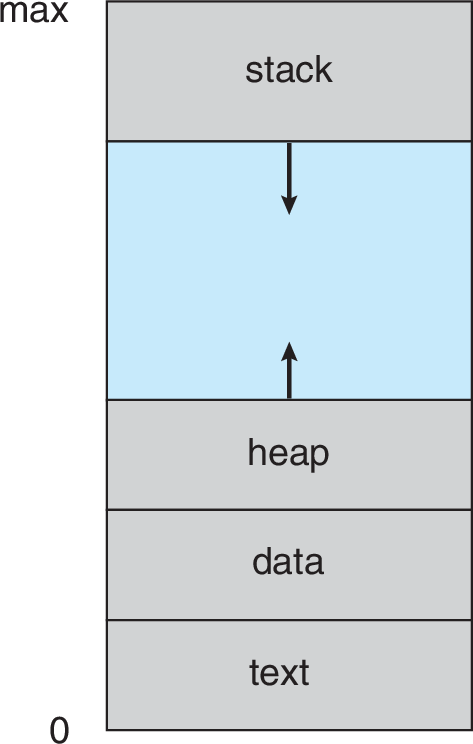
\includegraphics[width=3cm]{figs/01-3_01.pdf}
      \end{center}
    \end{column}
  \end{columns}
\end{frame}

%---------------------------------------------------------------------
\begin{frame}
  \frametitle{Estados}

  Un proceso en ejecución puede cambiar de estado.
  
    \begin{description}
      \item<2->[New] En creación
      \item<3->[Running] En ejecución
      \item<4->[Waiting] Esperando algún (E/S, señal)
      \item<5->[Ready] Listo para ejecutar. Esperando asignación de CPU
      \item<6->[Terminated] Ejecución terminada
    \end{description}

  \onslide<7->{
  \begin{center}

    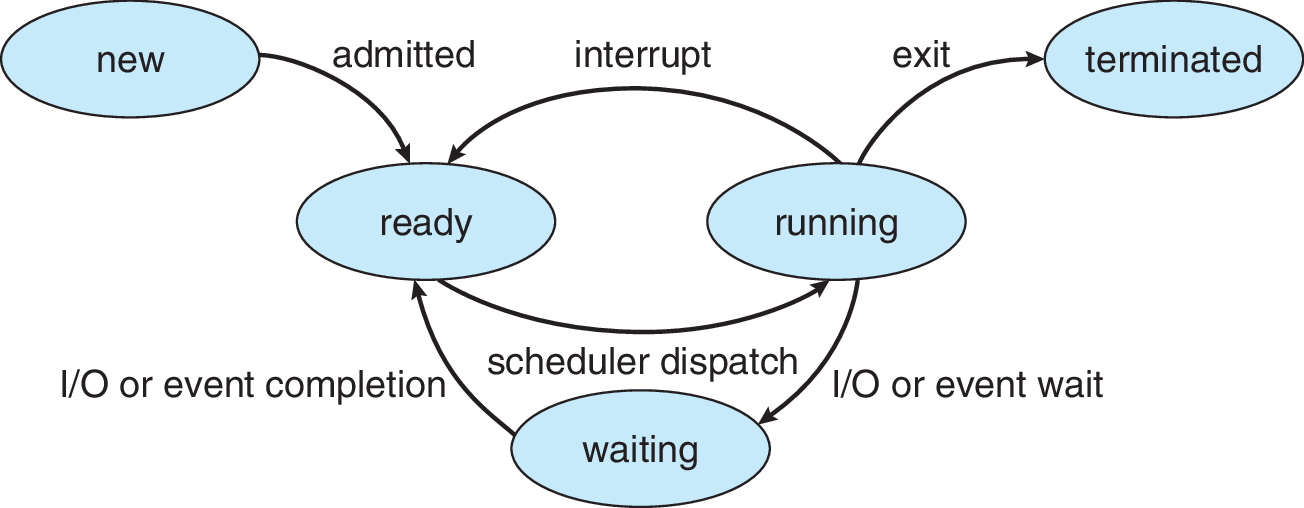
\includegraphics[width=8cm]{figs/01-3_02.pdf}
    
    \onslide<8->{¡Un autómata!}
  \end{center}
  }

\end{frame}

%---------------------------------------------------------------------
\begin{frame}[fragile]
  \frametitle{Estados}
  \framesubtitle{¿Cómo averiguo el estado de un proceso?}

  Con un script:
  \begin{minted}[mathescape,numbersep=5pt,gobble=2,frame=lines,framesep=2mm,fontsize=\scriptsize]{c}
  $ top
  $ htop
  $ ps aux
  \end{minted}

  Con un programa en C:
  \begin{minted}[mathescape,numbersep=5pt,gobble=0,frame=lines,framesep=2mm,fontsize=\scriptsize]{bash}
#include <sys/types.h>
#include <sys/wait.h>
int status;
pid_t return_pid = waitpid(process_id, &status, WNOHANG);
if (return_pid == -1) {
    /* error */
} else if (return_pid == 0) {
    /* child is still running */
} else if (return_pid == process_id) {
    /* child is finished. exit status in   status */
}
\end{minted}

  

\end{frame}
%---------------------------------------------------------------------
\begin{frame}
  \frametitle{Representación de Procesos}
  \framesubtitle{¿Cómo represento un proceso?}
  
  Estructura: {\bf Process Control Block (PCB)}

  \begin{columns}[c]
    \begin{column}[T]{8.5cm}
      \begin{itemize}
        \item<3-> Estado
        \item<4-> Identificador (PID)
        \item<5-> Program Counter (PC)
        \item<6-> Registros de CPU: {\em estado de ejecución}
        \item<7-> Información de {\em scheduling}: prioridades, tipo de cola, \ldots
        \item<8-> Información de memoria: límites, tabla de páginas/segmentos, \ldots
        \item<9-> Contabilidad ({\em accounting})
        \item<9-> Información de E/S: archivos y dispositivos abiertos, \ldots
      \end{itemize}
    \end{column}
    
    \begin{column}[T]{3cm}
      \onslide<2->{
      \begin{center}
        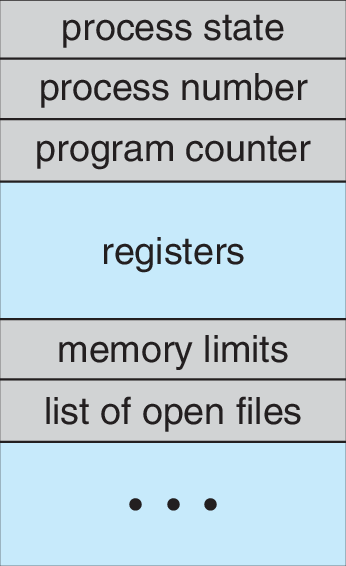
\includegraphics[width=3cm]{figs/01-3_03.pdf}
      \end{center}
      }
    \end{column}
  \end{columns}

  \onslide<10->{Miremos en {\tt include/linux/sched.h}}
  
\end{frame}


%---------------------------------------------------------------------

\begin{frame}
  \frametitle{Cambio de un proceso a otro}
  \framesubtitle{{\em Context Switch}}
  
  \begin{center}
    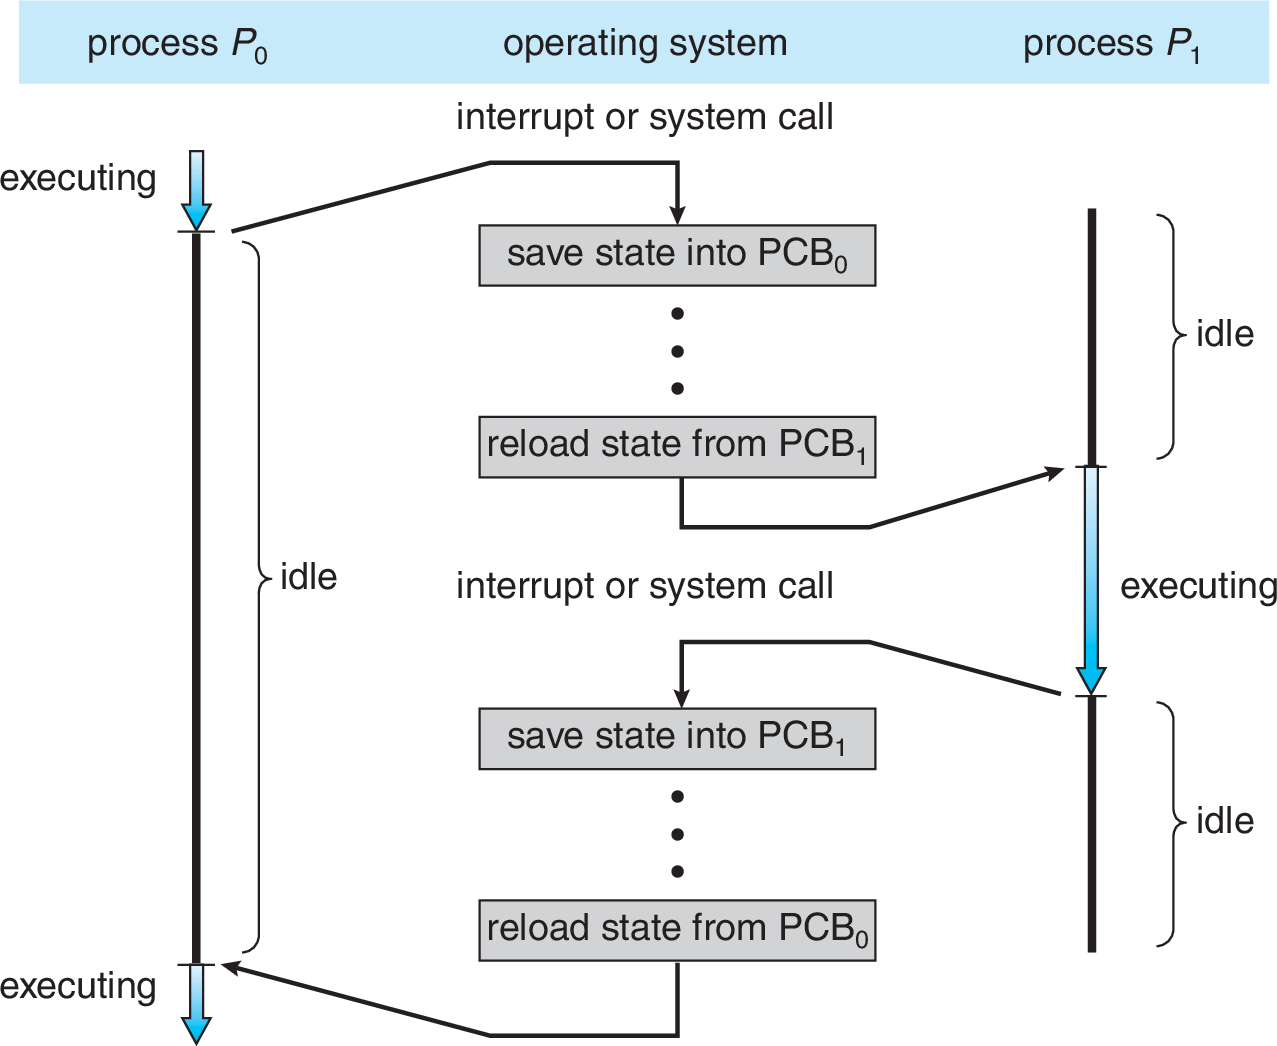
\includegraphics[width=8cm]{figs/01-3_04.pdf}
  \end{center}

\end{frame}


%---------------------------------------------------------------------
\subsection{Manipulando procesos}

\begin{frame}
  \frametitle{Operaciones sobre procesos}
  \framesubtitle{Creación de procesos: ¿el huevo o la gallina?}
  ¿Quién crea un proceso? \onslide<2->{\ldots otro proceso}
  \onslide<3->{¿Quién crea ese otro proceso?} \onslide<4->{\ldots otro proceso}
  \onslide<5->{¿Quién crea ese otro proceso?} \onslide<6->{\ldots otro proceso}

  \begin{itemize}
    \item<7->Linux: {\tt init} ({\bf pid}=1)
    \item<7->MacOS X: {\tt launchd} ({\bf pid}=1)
    \item<7->Windows: {\tt InitialSystemProcess}, ó {\tt System} ({\bf pid}=4)
  \end{itemize}

  \onslide<8->{Procesos que crea otro {\bf \ldots es su padre}}
  \begin{itemize}
    \item<9-> Se forma un {\bf árbol de procesos}
    \item<9-> Procesos tienen un {\bf pid} y un {\bf ppid} (parent pid)
    \item<10-> Probemos {\tt pstree}
  \end{itemize}
\end{frame}

%---------------------------------------------------------------------
\begin{frame}
  \frametitle{Creando procesos}
  \framesubtitle{OK, hemos creado un proceso hijo \ldots ¿y ahora?}

  ¿Quién sigue ejecutando? (modos de ejecución)
  \begin{itemize}
    \item Padre e hijo continúan ejecutando concurrentemente
    \item Padre espera que algunos o todos sus hijos terminen
  \end{itemize}

  ¿Qué personalidad tiene el hijo? (modos de espacio de direcciones)
  \begin{itemize}
    \item El hijo es un duplicado del padre (sección {\em code} y {\em data} son copiadas)
    \item El hijo es un nuevo programa
  \end{itemize}

\end{frame}

%---------------------------------------------------------------------
\begin{frame}
  \frametitle{Creando procesos}
  \framesubtitle{{\tt fork()} y {\tt exec()} son buenos amigos (y por eso casi siempre se ejecutan unidos)}
  
  \begin{block}{{\tt fork()} syscall}
    \onslide<2->{
    Crea un nuevo proceso como {\bf copia} del padre.
    Ambos continúan ejecutando desde la instrucción posterior a {\tt fork}
    }
    
    \onslide<3->{¿Cómo distinguirlos?}
    \begin{itemize}
      \item<4-> En el padre, {\tt fork()} retorna el {\bf pid} del hijo
      \item<4-> En el hijo, {\tt fork()} retorna 0
    \end{itemize}
  \end{block}
  
  \begin{block}{{\tt exec()} syscall}
    \onslide<5->{Carga un binario en memoria {\bf reemplazando} el código de quien lo llamó, e inicia su ejecución.}
  \end{block}
\end{frame}

%---------------------------------------------------------------------
\begin{frame}
  \frametitle{Creando procesos}
  \framesubtitle{{\tt fork()} y {\tt exec()} \ldots son buenos amigos (y por eso casi siempre se ejecutan unidos)}

  Usualmente, después del {\tt fork()}, uno de los dos (el hijo) ejecuta un {\tt exec()}.

  \begin{itemize}
    \item El padre conoce el {\bf pid} del hijo
    \item El padre podría seguir ejecutando y crear más hijos
    \item \ldots o bien esperar que el hijo termine (o muera) ejecutando el syscall {\tt wait()}
  \end{itemize}

  \begin{center}
    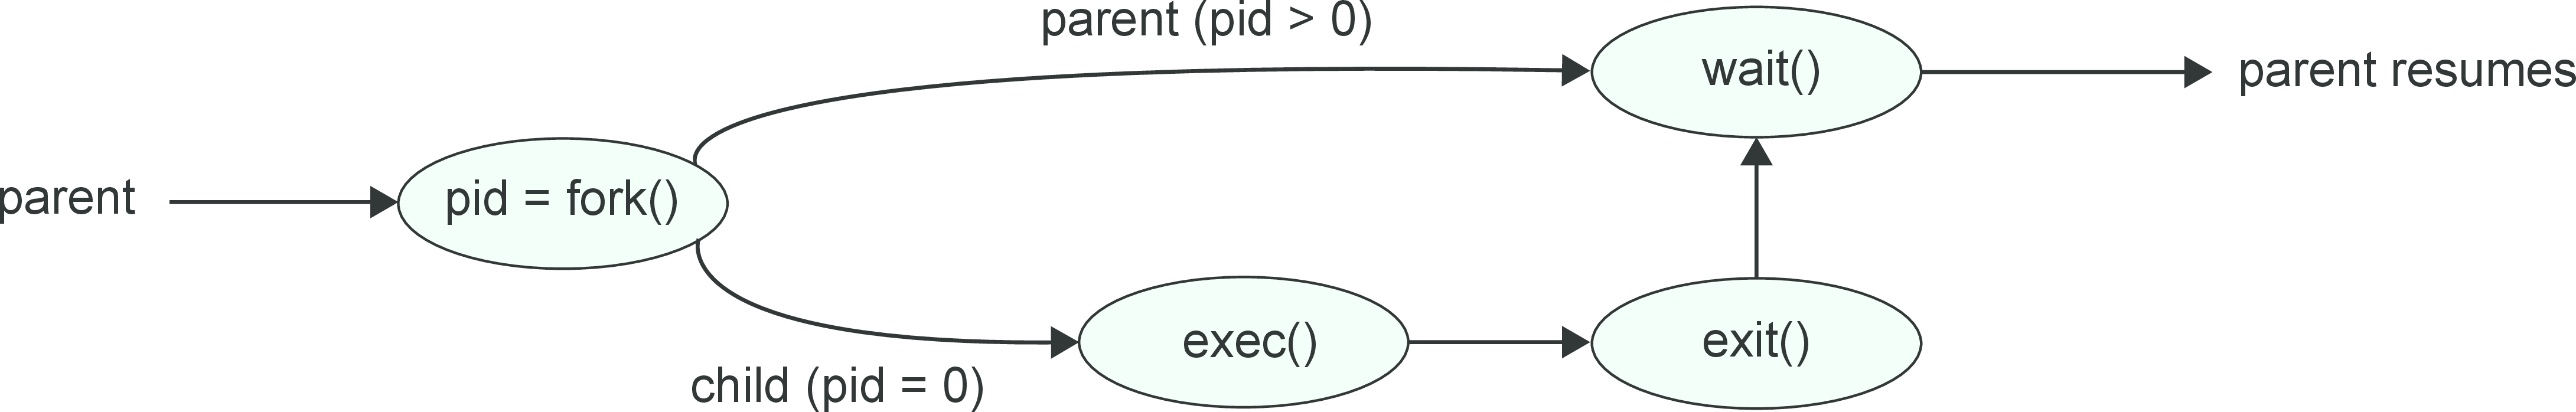
\includegraphics[width=11cm]{figs/01-3_10.pdf}
  \end{center}
  

\end{frame}

%---------------------------------------------------------------------
\begin{frame}[fragile]
  \frametitle{Creando procesos}
  \framesubtitle{Ejemplo de {\tt fork()}}

\begin{minted}[mathescape,numbersep=5pt,gobble=2,frame=lines,framesep=2mm,fontsize=\scriptsize]{c}
  int main() {
    pid_t childpid; /* variable to store the child's pid */
    int status;     /* parent process: child's exit status */
    int a = 42;
    childpid = fork(); /* now create new process */
    if (childpid == 0) { /* fork() returns 0 to the child process */
            a++;
            printf("CHILD: I am the child process!\n");
            printf("CHILD: The value of a is : %d\n", a);
            exit(50); /* child exits with return code 50 */
    }
    else if(childpid > 0) { /* fork() returns new pid to the parent process */
            printf("PARENT: I am the parent process!\n");
            printf("PARENT: The value of my copy of childpid is %d\n", childpid);
            wait(&status); /* wait for child to exit, and store its status */
            printf("PARENT: Child's exit code is: %d\n", status);
            printf("PARENT: The value of a is : %d\n", a);
            exit(0);  /* parent exits */
    }
    return 0;
  }
\end{minted}

\end{frame}

%---------------------------------------------------------------------
\begin{frame}[fragile]
  \frametitle{Creando procesos}
  \framesubtitle{Ejemplo de {\tt fork()}}

¿Cuántos procesos se crean con este código?

\begin{minted}[mathescape,numbersep=5pt,gobble=2,frame=lines,framesep=2mm,fontsize=\scriptsize]{c}
  int main(int argc, char *arg[]) {
    int pid;
    int i=0;
    for(i=0; i<4; i++) {
      fork();
      printf("%d\n", i);
    }
    return 0;
  }
\end{minted}
\end{frame}


%---------------------------------------------------------------------
\begin{frame}
  \frametitle{Terminando procesos}
  \framesubtitle{{\tt exit()} $\equiv$ ``kill me'', {\tt kill()} $\equiv$ ``kill somebody''}

  \begin{block}{{\tt exit()} syscall}
  Todo proceso, al terminar su ejecución, ejecuta {\tt exit()}
  \begin{itemize}
     \item<2-> Adicionalmente entrega un {\em código de retorno} (¿para qué?) al padre.
     \item<2-> Sistema Operativo recupera todos los recursos asignados
  \end{itemize}
  \end{block}  

  \onslide<3->{
  \begin{block}{{\tt kill()} syscall ({\tt TerminateProcess()})}  
  Permite enviar una señal a {\bf otro} proceso (típicamente {\tt SIGTERM})
  \begin{itemize}
    \item<4-> La señal SIGKILL efectivamente mata el proceso.
  \end{itemize}
  \end{block}
  }
\end{frame}

%---------------------------------------------------------------------
\begin{frame}[fragile]
  \frametitle{Terminando procesos}
  \framesubtitle{Si el padre muere, ¿deben morir los hijos?}

  Usualmente el sistema operativo no permite que un hijo exista si el padre ha terminado.
  \begin{itemize}
    \item Sistema Operativo ejecuta una {\bf terminación en cascada}
  \end{itemize}
  
  ¿Cómo se hace en Linux? \onslide<2->{Proceso termina:
  \begin{center}
    {\tt exit(1);}
  \end{center}
  }
  
  \onslide<3->{Padre recupera el estado del hijo ejecutando:}
\begin{minted}[mathescape,numbersep=5pt,gobble=2,frame=lines,framesep=2mm,fontsize=\scriptsize]{c}
     pid_t pid;
     int status;
     pid = wait(&status);
\end{minted}

  \onslide<4->{Padre ha recibido el status en {\tt status} }
\end{frame}

%---------------------------------------------------------------------
\begin{frame}
  \frametitle{Terminando procesos}
  \framesubtitle{Huérfanos y zombies: the walking process}

  Proceso terminado no se borra inmediatamente de la tabla de procesos.
  
  ¿Por qué? \onslide<2->{Para que el padre recupere su estado de salida con {\tt wait()}}

  \begin{itemize}
    \item<3-> Procesos terminados son {\bf zombies} hasta que su padre hace {\tt wait()}
    \item<4-> Cuando el padre hace {\tt wait()} la entrada del hijo se borra de la tabla
  \end{itemize}

  \onslide<5->{¿Y si el padre jamás hace {\tt wait()}?}
  \begin{itemize}
    \item<6->Si el padre termina sin ejecutar {\tt wait()}, el hijo queda {\bf huérfano}.
    \item<7->Linux/UNIX: huérfanos pasan a ser hijos de {\tt init}
    \item<7->{\tt init} llama periódicamente a {\tt wait()} para deshacerse de los huérfanos.
  \end{itemize}

\end{frame}

%---------------------------------------------------------------------
\begin{frame}[fragile]
  \frametitle{Creando zombies}

\begin{minted}[mathescape,numbersep=5pt,gobble=0,frame=lines,framesep=2mm,fontsize=\scriptsize]{c}
#include<sys/wait.h>
#include<stdlib.h>
#include<unistd.h>

int main(void) {
  pid_t pids[10];
  int i;
  for (i = 9; i >= 0; --i) {
    pids[i] = fork();
    if (pids[i] == 0) {
       sleep(i+1);
       exit(0);
    }
  }
  for (i = 9; i >= 0; --i)
    waitpid(pids[i], NULL, 0);
  return 0;
}
\end{minted}
\end{frame}

%---------------------------------------------------------------------
\subsection{Comunicación entre procesos (IPC)}

\begin{frame}
  \frametitle{{\em InterProcess Comunication (IPC)}}

  Si hay multiprogramación, hay múltiples procesos ``en ejecución''\footnote{ya sabemos que esto no es estrictamente correcto}

  \onslide<2->{Procesos {\bf independientes} no provocan problemas \ldots}
  \onslide<3->{procesos {\bf cooperativos} requieren {\bf comunicación inter-procesos}}
  
  \onslide<4->{Dos modelos fundamentales de IPC:}
  \begin{itemize}
    \item<5-> {\bf Memoria compartida} ({\em shared memory})
    \item<5-> {\bf Paso de mensajes} ({\em message passing})
  \end{itemize}
  
\end{frame}

%---------------------------------------------------------------------
\begin{frame}
  \frametitle{Memoria compartida vs. Paso de mensajes}
  \framesubtitle{Fight!}
  
  \begin{block}{Memoria compartida}
    \onslide<2->{Procesos acuerdan un espacio de memoria donde ambos pueden escribir}
    \begin{itemize}
      \item<4->Más rápido que paso de mensajes (sólo un {\em syscall} para crearla)
      \item<6->Requiere coordinar accesos
    \end{itemize}
  \end{block}

  \begin{block}{Paso de mensajes}
    \onslide<3->{Procesos se envían mensajes}
    \begin{itemize}
      \item<5->Requiere {\em syscall}s {\tt send}/{\tt recv}
      \item<7->Fácil de programar para envíos pequeños (no provoca conflictos)
    \end{itemize}
  \end{block}


\end{frame}

%---------------------------------------------------------------------
\begin{frame}
  \frametitle{Memoria compartida vs. Paso de mensajes}
  \framesubtitle{Fight!}

  \begin{center}
    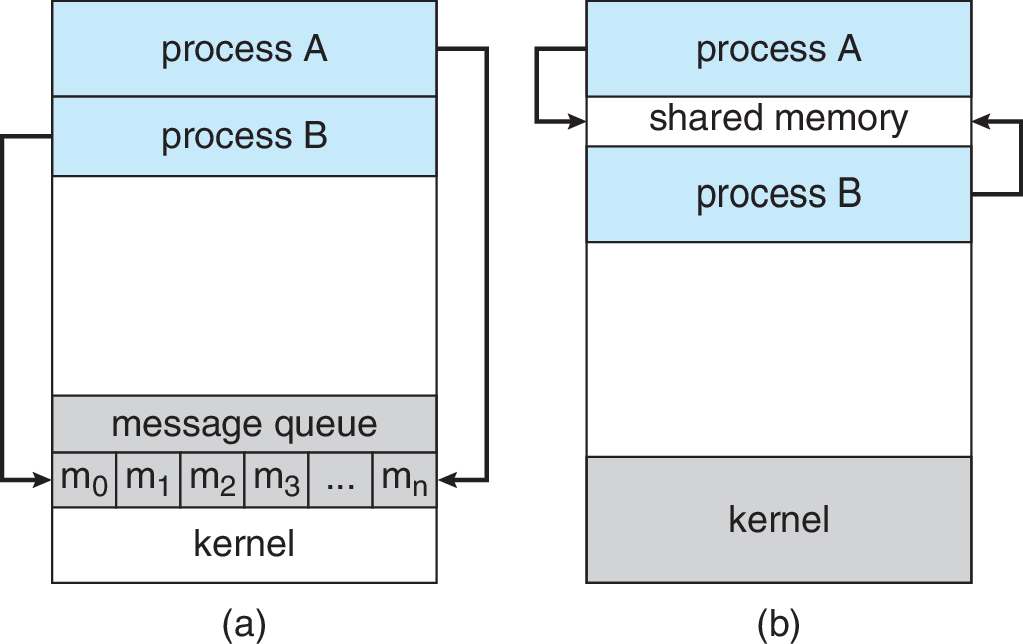
\includegraphics[width=8cm]{figs/01-3_12.pdf}
  \end{center}




\end{frame}
%---------------------------------------------------------------------
\begin{frame}
  \frametitle{Memoria compartida}
  \framesubtitle{{\em Shared Memory}}

  ¿Escribir en memoria de otro proceso?
  \begin{itemize}
    \item<2-> Procesos $A$ y $B$ deben {\bf acordar} permitirse acceso
    \item<2-> Proceso $A$ designa una región de su espacio de memoria como {\em compartida}
    \item<2-> Proceso $B$ agrega esa región como parte de su espacio
    \item<2-> $A$ y $B$ se preocupan de coordinar los accesos
  \end{itemize}

  \onslide<3->{
  API POSIX provee syscall para crear y exponer regiones de memoria compartida
  \begin{itemize}
    \item<4-> {\em Memory-mapped files}
    \item<4-> {\tt shm\_open()}, {\tt ftruncate()}, {\tt mmap()}, {\tt shm\_unlink()}
  \end{itemize}
  }
\end{frame}

%---------------------------------------------------------------------
%\begin{frame}
%  \frametitle{Un problema clásico de coordinación}
%  
%  \begin{block}{Problema del productor y consumidor}
%    Proceso {\bf productor} produce información.
%    
%    Proceso {\bf consumidor} consume información del productor.
%  \end{block}
%  
%  \begin{center}
%    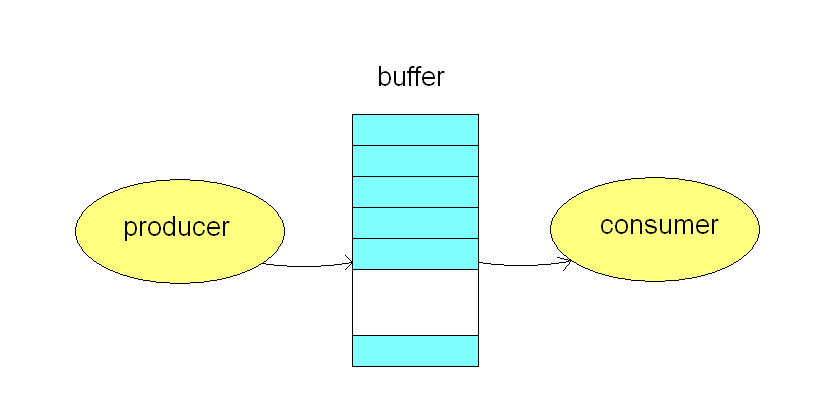
\includegraphics[width=8cm]{figs/01-ProdCons.png}
%  \end{center}
%
%  Variantes: {\bf buffer limitado} ó {\bf ilimitado}
%  \begin{itemize}
%    \item Con {\bf buffer limitado} el productor puede tener que esperar
%  \end{itemize}
%\end{frame}
%
%---------------------------------------------------------------------
%\begin{frame}[fragile]
%  \frametitle{Memoria compartida}
%  \framesubtitle{{\em Shared Memory}}
%
%  Buffer limitado ({\em bounded}) en memoria compartida
%  
%\begin{minted}[mathescape,numbersep=5pt,gobble=2,frame=lines,framesep=2mm,fontsize=\scriptsize]{c}
%  #define BUFFER_SIZE 10
%  
%  typedef struct {
%     ...
%  } item;
%  
%  item buffer[BUFFER_SIZE];
%  int in = 0;     // proxima posicion libre
%  int out = 0;    // primera posicion llena
%\end{minted}
%
%¿Cuándo está lleno el buffer? ¿Cuándo está vacío?
%  
%\end{frame}

%---------------------------------------------------------------------
%\begin{frame}[fragile]
%  \frametitle{Memoria compartida}
%  \framesubtitle{{\em Shared Memory}}
%
%  \begin{center}
%    Proceso {\bf productor}
%  \end{center}
%
%\begin{minted}[mathescape,numbersep=5pt,gobble=2,frame=lines,framesep=2mm,fontsize=\scriptsize]{c}
%  item next_product;
%  
%  while(true) {
%    next_product = produce();
%    while ( ((in+1)%BUFFER_SIZE) == out);
%    
%    buffer[in] = next_product;
%    in = (in+1)%BUFFER_SIZE;
%  }
%\end{minted}
%
%\end{frame}

%---------------------------------------------------------------------
%\begin{frame}[fragile]
%  \frametitle{Memoria compartida}
%  \framesubtitle{{\em Shared Memory}}
%
%  \begin{center}
%    Proceso {\bf consumidor}
%  \end{center}
%
%\begin{minted}[mathescape,numbersep=5pt,gobble=2,frame=lines,framesep=2mm,fontsize=\scriptsize]{c}
%  item next_consumed;
%  
%  while(true) {
%    while(in == out);
%    
%    next_consumed = buffer[out];
%    out = (out+1)%BUFFER_SIZE;
%    
%    consume(next_consumed);
%  }
%\end{minted}
%
%  ¿Cuántos ítemes puede haber como máximo en el {\em buffer}?
%\end{frame}
%
%---------------------------------------------------------------------
\begin{frame}
  \frametitle{Paso de mensajes}
  \framesubtitle{{\em Message Passing}}

  Abstracción de {\em mensaje}. Dos primitivas:
  \begin{itemize}
    \item {\tt send(message)}
    \item {\tt receive(message)}
  \end{itemize}
  ¿Cómo habilitar la comunicación? Varios aspectos a decidir
  \begin{itemize}
    \item Comunicación directa o indirecta
      \begin{itemize}
        \item {\tt send(P, message)}, {\tt recv(Q, message)}, {\tt recv(\&id, message)}
        \item {\tt send(A, message)}, {\tt recv(A, message)}
      \end{itemize}
    \item Comunicación síncrona o asíncrona
    %\item {\em Buffered} ó {\em unbuffered}
  \end{itemize}

\end{frame}
%%---------------------------------------------------------------------
%\begin{frame}
%  \frametitle{Paso de mensajes}
%  \framesubtitle{Comunicación directa vs indirecta}
%  
%  Con {\bf comunicación directa}, cada proceso debe conocer el {\em nombre} del otro
%  \begin{itemize}
%    \item {\tt send(P, message)}
%    \item {\tt receive(Q, message)}
%  \end{itemize}
%  Este esquema es {\bf simétrico}
%  \begin{itemize}
%    \item {\tt receive(\&id, message)}. Variante {\em asimétrica}.
%  \end{itemize}
%
%  Con {\bf comunicación indirecta} utiliza abstracción de {\em mailbox} o {\em port}
%  \begin{itemize}
%    \item {\tt send(A, message)}
%    \item {\tt receive(A, message)}
%  \end{itemize}
%  Ambos deben poseer un referencie a la {\em mailbox} {\tt A}
%\end{frame}

%---------------------------------------------------------------------
%\begin{frame}
%  \frametitle{Paso de mensajes}
%  \framesubtitle{Comunicación síncrona vs asíncrona}
%
%  Tanto {\tt send()} como {\tt receive()} pueden ser {\bf bloqueantes} (síncrono)
%  o {\bf no bloqueantes} (asíncrono)
%
%  \begin{itemize}
%    \item {\tt send} {\bf bloqueante}: bloquea hasta que el mensaje es recibido
%    \item {\tt send} {\bf no-bloqueante}: envía y continúa
%    \item {\tt recv} {\bf bloqueante}: espera hasta recibir un mensaje
%    \item {\tt recv} {\bf no-bloqueante}: recibe un mensaje inmediatamente o {\tt null}
%  \end{itemize}
%
%\end{frame}

%---------------------------------------------------------------------
%\begin{frame}
%  \frametitle{Paso de mensajes}
%  \framesubtitle{Comunicación {\em buffered} ó {\em unbuffered}}
%
%  Sistemas Operativos usan {\em colas} temporales para transmitir mensajes
%  \begin{itemize}
%    \item {\bf Cola de capacidad cero}: fuerza {\tt send()} bloqueante
%    \item {\bf Cola de capacidad limitada}: máximo de $n$ mensajes encolados mientras no sean recibidos.
%          Si se llena, el siguiente {\tt send()} se bloquea
%    \item {\bf Cola de capacidad ilimitada}: cola potencialmente infinita
%  \end{itemize}
%  
%\end{frame}

%---------------------------------------------------------------------
%\begin{frame}
%  \frametitle{Más comunicación inter-procesos}
%  \framesubtitle{Algunas técnicas de más alto nivel}
%
%  {\bf Sockets}: punto de comunicación de servicios
%  \begin{itemize}
%    \item Indexado por enteros
%    \item Comunicación cliente/servidor
%    \item Para comunicación TCP ó UDP\footnote{Si no sabe que es esto, búsquelo en Google o espere hasta los capítulos de redes}
%  \end{itemize}
%
%  \begin{center}
%    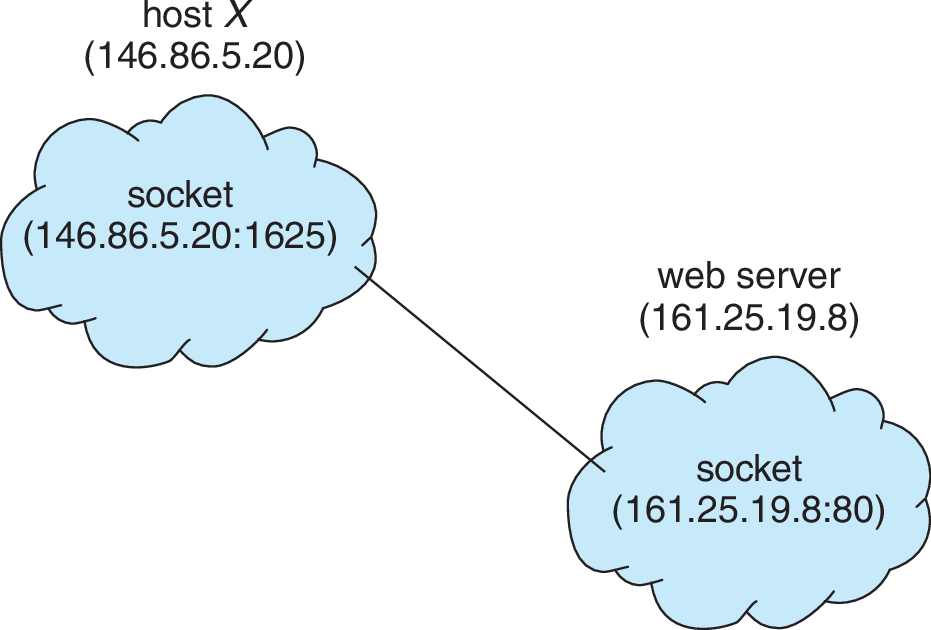
\includegraphics[width=6cm]{figs/01-3_20.pdf}
%  \end{center}
%
%\end{frame}


%---------------------------------------------------------------------
%\begin{frame}
%  \frametitle{Más comunicación inter-procesos}
%  \framesubtitle{Algunas técnicas de más alto nivel}
%
%  {\bf RPC}: Remote Procedure Call\footnote{Más de esto en IIC2523, Sistemas Distribuidos}
%  \begin{itemize}
%    \item Comunicación a nivel de funciones (métodos) en otro proceso
%    \item Requiere un intermediario ({\em matchmaker/portmapper}) para ubicar los proveedores del método remoto
%    \item Versión {\em object oriented}: {\bf RMI}, {\em Remote Method Invocation}
%    \item Mismo esquema usado por {\em Web Services}
%  \end{itemize}
%  
%  \begin{center}
%    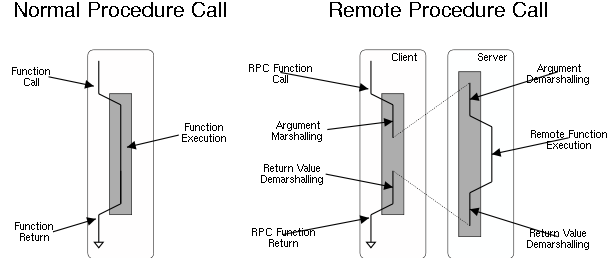
\includegraphics[width=6cm]{figs/01-RPC.png}
%  \end{center}
%
%\end{frame}
%
%---------------------------------------------------------------------
\begin{frame}
  \frametitle{Más comunicación inter-procesos}
  \framesubtitle{Algunas técnicas de más alto nivel}

  {\bf Pipes}: {\em tubo} entre dos procesos
  \begin{itemize}
    \item Unidireccionales o bidireccionales
    \item Un proceso escribe en un extremo ({\em write-end}), y otro proceso lee desde el otro extremo ({\em read-end})
    \item Pueden ser tratadas como archivos
    \item Implementacióm implícitas en consolas. Ej: {\tt ls | more}
  \end{itemize}

  \begin{center}
    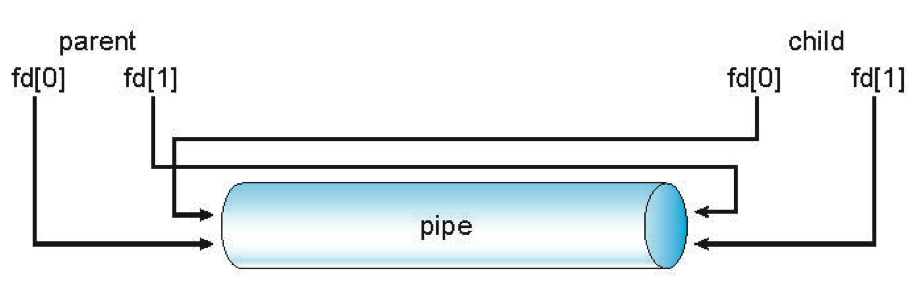
\includegraphics[width=10cm]{figs/01-pipes.png}
  \end{center}

\end{frame}

%---------------------------------------------------------------------
\begin{frame}
  \frametitle{Resumen: Procesos}
  \framesubtitle{Algunos puntos clave}

  \begin{block}{Procesos}
    \begin{itemize}
    \item Programa en ejecución + recursos
    \item Pasan por estados
    \item Representados por PCBs
    \item Proceso que no está en ejecución se mantiene en una cola
    %\item {\em Scheduler} decide qué proceso debe ejecutar
    \item Pueden crear otros procesos, estableciendo relación {\em padre-hijo}
    \item Pueden comunicarse usando varios métodos
    \end{itemize}
  \end{block}

\end{frame}
%---------------------------------------------------------------------
\begin{frame}
  \frametitle{Desafío \#1: Fork de Procesos}
  %\framesubtitle{Algunos puntos clave}

  \begin{enumerate}
    \item Entrar a sitio del curso en \url{http://edx.ing.puc.cl}.
    \item Construir un código único en C que cree un proceso que permita crear un árbol binario de procesos
          con $3$ niveles.
      \begin{itemize}
        \item Nivel 1: Proceso padre, $P_0$ crea dos hijos $P_1$, $P_2$
        \item Nivel 2: $P_1$ y $P_2$ crean dos hijos cada uno
        \item Nivel 3: Procesos hoja imprimen su PID, su PPID, y un mensaje de despedida.
        \item Cada proceso padre debe esperar a los hijos
        \item Cuando todos los descendientes han terminado, el padre debe mostrar la hora actual ({\tt date})
        \item Bonus si funciona para $N$ niveles
      \end{itemize}
    \item Plazo: 18-Agosto-2015, 23:59.
    \item Pueden hacerlo en conjuntos de $N$, $1 \leq N \leq 3$.
  \end{enumerate}
\end{frame}


%---------------------------------------------------------------------
\section{{\em Threads}}

\subsection{{\em Threads} y {\em Multicores}}

\begin{frame}
  \frametitle{{\em Threads}}

  {\em {\bf Thread}}: Como un proceso, pero más liviano.
  
  \onslide<2->{Unidad básica de uso de CPU}
  
  \onslide<3->{Le trae:
  \begin{itemize}
    \item {\em Thread ID} ({\bf tid})
    \item Program Counter
    \item Registros
    \item {\em Stack}
  \end{itemize}
  }
  
  \onslide<4->{¿y el resto?} \onslide<5->{\ldots compartido con un proceso}
  
\end{frame}

%---------------------------------------------------------------------
\begin{frame}
  \frametitle{ {\em Single-threading} vs {\em Multi-threading}}
  
  Procesos pueden tener uno o más {\em threads}
  
  \begin{center}
    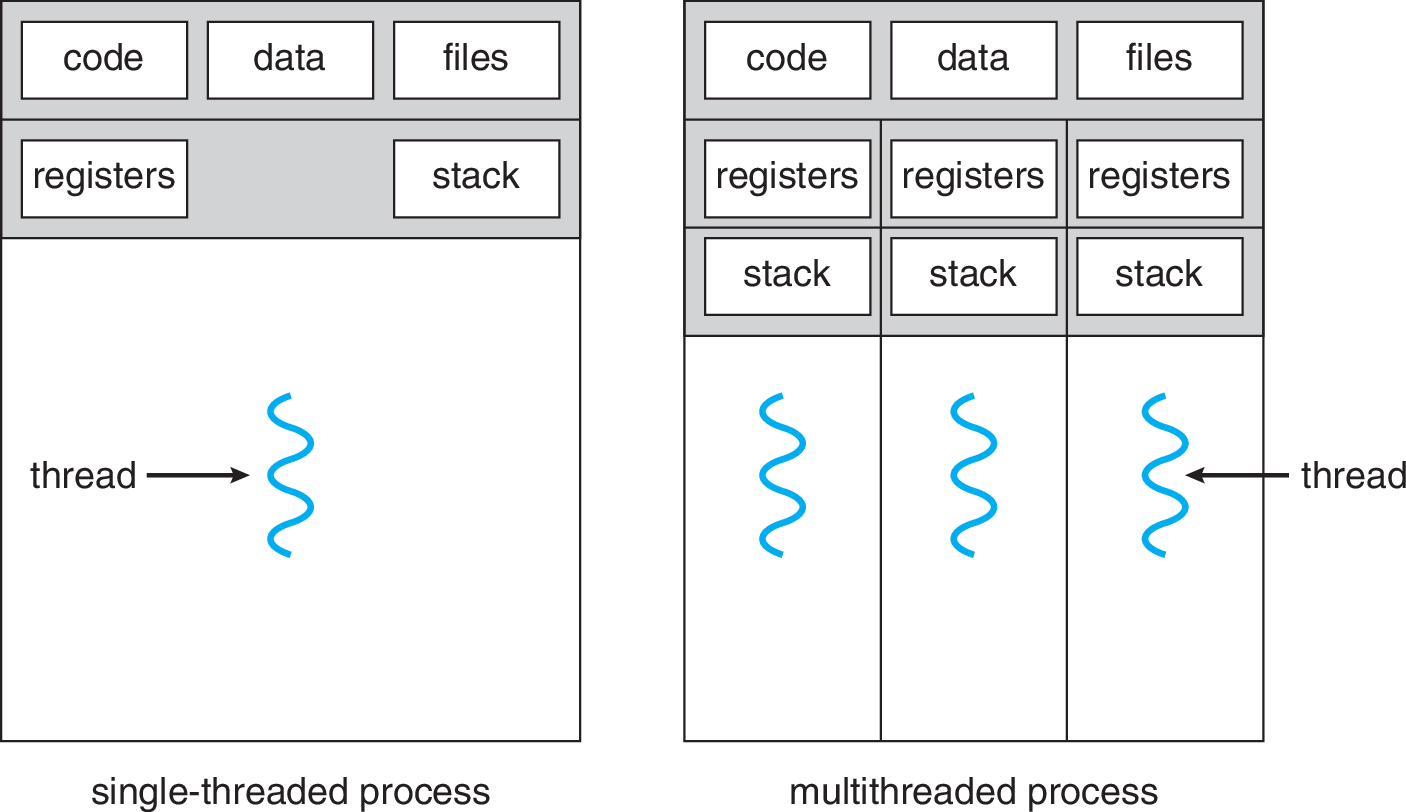
\includegraphics[width=10cm]{figs/01-4_01.pdf}
  \end{center}  
  
\end{frame}

%---------------------------------------------------------------------
%\begin{frame}
%  \frametitle{ {\em Multi-threading}}
%  \framesubtitle{¿Para qué?}
%  
%  \begin{itemize}
%    \item Proceso son unidades {\em pesadas}
%    \item {\em Threads} pueden ejecutar parte del código de un proceso
%      \begin{itemize}
%        \item Concurrencia real en la medida que hayan múltiples {\em core}s
%      \end{itemize}
%    \item Un {\em web browser} puede:
%      \begin{itemize}
%        \item Recuperar y desplegar imágenes
%        \item Hacer {\em parsing} de HTML
%        \item Proponer opciones de autocompletado mientras se escribir
%        \item Ejecutar corrector ortográfico mientras se escribe
%      \end{itemize}
%  \end{itemize}
%
%  Si voy a ejecutar parte del mismo código, talvez no necesito crear un proceso nuevo.
%  
%  Es como hacer {\tt fork()} ¿y \ldots hacer {\tt exec()}?
%
%\end{frame}
%
%%---------------------------------------------------------------------
%\begin{frame}
%  \frametitle{ {\em Multi-threading}}
%  \framesubtitle{¿Para qué?}
%
%  Otro caso: un {\em web server} necesita atender múltiples conexiones
%  \begin{itemize}
%    \item ¿Espero atender completamente una antes de recibir la siguiente?
%  \end{itemize}
%
%  \begin{center}
%    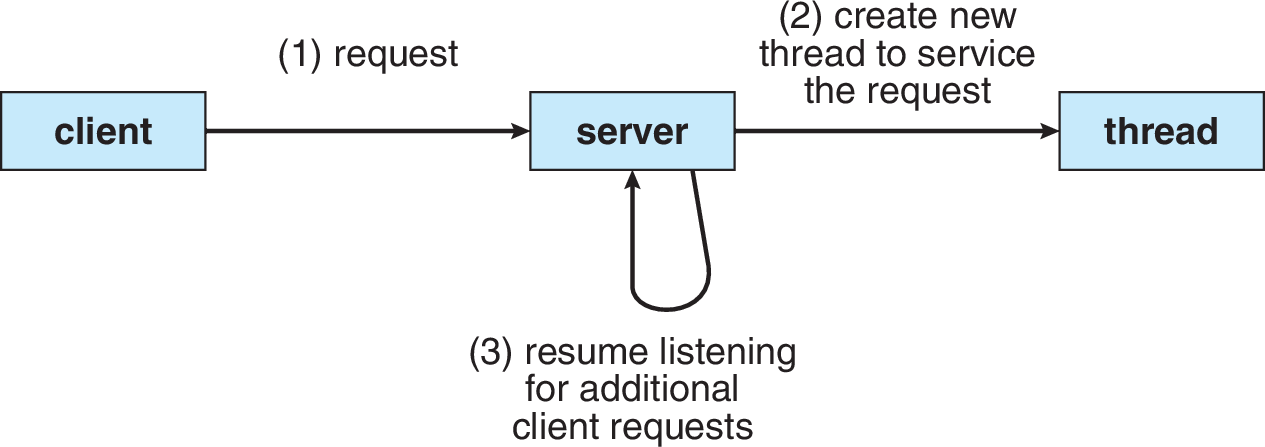
\includegraphics[width=10cm]{figs/01-4_02.pdf}
%  \end{center}  
%
%\end{frame}

%---------------------------------------------------------------------
\begin{frame}
  \frametitle{ {\em Multi-cores} y {\em Multi-threading}}

  Con {\em single-core} solo un {\em thread} de un proceso puede ejecutar al mismo tiempo

  %\onslide<2->{¿Cómo se provee la ilusión de que múltiples {\em threads} ejecutan simultáneamente? }
  
  \onslide<2->{\ldots ¡pero ahora hay {\bf multi-core}s!}
  
  \begin{itemize}
    \item<3-> Múltiples {\em threads} avanzan: {\bf concurrencia}
    \item<3-> Múltiples {\em threads} ejecutan simultáneamente: {\bf paralelismo}
  \end{itemize}
  
\end{frame}

%---------------------------------------------------------------------
\begin{frame}
  \frametitle{ {\em Multi-cores} y {\em Multi-threading}}
  \framesubtitle{¿Cuánto gano?}
  
  Gene Amdahl propuso una fórmula (1967) para calcular la mejora {\em potencial} de un programa
  que contiene partes paralelizables y partes secuenciales
  
  \begin{equation*}
    \mathit{speedup} \leq \frac{1}{S + \frac{(1-S)}{N}}
  \end{equation*}
  
  $S$: Porción de código que debe ser ejecutado de manera secuencial
  
  $N$: Número de {\em core}s
  
  El {\em speedup} es un valor positivo que indica la mejora de un código paralelo respecto a su versión secuencial
  
  \begin{equation*}
    \mathit{speedup} = \frac{T_{\mathit{secuencial}}}{T_{\mathit{paralelo}}} = \frac{T_{1}}{T_{N}}
  \end{equation*}
  
  Ejemplo: $\mathit{speedup}=2$ signfica que $T_{1}=2T_{N}$, esto es, dos veces más rápido
\end{frame}
%---------------------------------------------------------------------
\begin{frame}
  \frametitle{Derivación de la Ley de Amdhal}
  \framesubtitle{(opcional)}

  Sea $T_N$ el tiempo de ejecución con $N$ cores, y $S$ la fracción de código que es estrictamente secuencial
  ($0 \leq S \leq 1$).
  
  El tiempo en $N$ cores se puede definir como:
  
  \begin{equation*}
    T_N = T_1 S + \frac{T_1}{N} (1-S) = T_1 \left( S + \frac{1-S}{N} \right)
  \end{equation*}
  
  Por lo tanto el {\em speedup} es:
  
  \begin{equation*}
    \mathit{speedup} = \frac{T_1}{T_N} = \frac{T_1}{T_1 \left( S + \frac{1-S}{N} \right)} = \frac{1}{S + \frac{1-S}{N}}
  \end{equation*}
  

\end{frame}

%---------------------------------------------------------------------
\begin{frame}
  \frametitle{ {\em Multi-threading} }
  \framesubtitle{¿Fácil?}

  Surgen desafíos para poder aprovechar el {\em multithreading}
  \begin{description}
    \item[División de tareas]<2-> ¿Qué tareas ejecuto en paralelo? Ideal: que sean independientes
    \item[Balance de carga]<2-> Idealmente: tareas de tamaño similar
    \item[División de datos]<2-> ¿Bajo qué criterio divido los datos entre {\em threads}?
    \item[Dependencias de datos]<2-> ¿Hay competencia por datos? ¿Necesito sincronizar accesos? ¿Puedo perder concurrencia?
    \item[Testing + Debugging]<2-> ¿Cómo {\em debuggear} una aplicación {\em multithreaded}?
  \end{description}

\end{frame}


%---------------------------------------------------------------------
\subsection{Modelos de {\em multithreading}}

\begin{frame}
  \frametitle{ Modelos de {\em Multi-threading} }

  Dos tipos de {\em threads}
  
  \begin{itemize}
    \item {\bf User threads}
      \begin{itemize}
        \item Manejados por una biblioteca de usuario
        \item Sistema Operativo sólo ve procesos
      \end{itemize}
    \item {\bf Kernel threads}
      \begin{itemize}
        \item Administrador por el Sistema Operativo (asignables a {\em core}s)
        \item Soportados en (casi) todos los Sistemas Operativos contemporáneos
      \end{itemize}
  \end{itemize}
  
  ¿Cómo se relacionan {\em kernel} y {\em user threads}?

\end{frame}

%---------------------------------------------------------------------
\begin{frame}
  \frametitle{ {\em Many-to-one} }
  
  \begin{itemize}
    \item + Manejo de {\em threads} en biblioteca de usuario
    \item - Un {\em syscall} de un {\em thread} bloquea todo el proceso
  \end{itemize}

  \begin{center}
    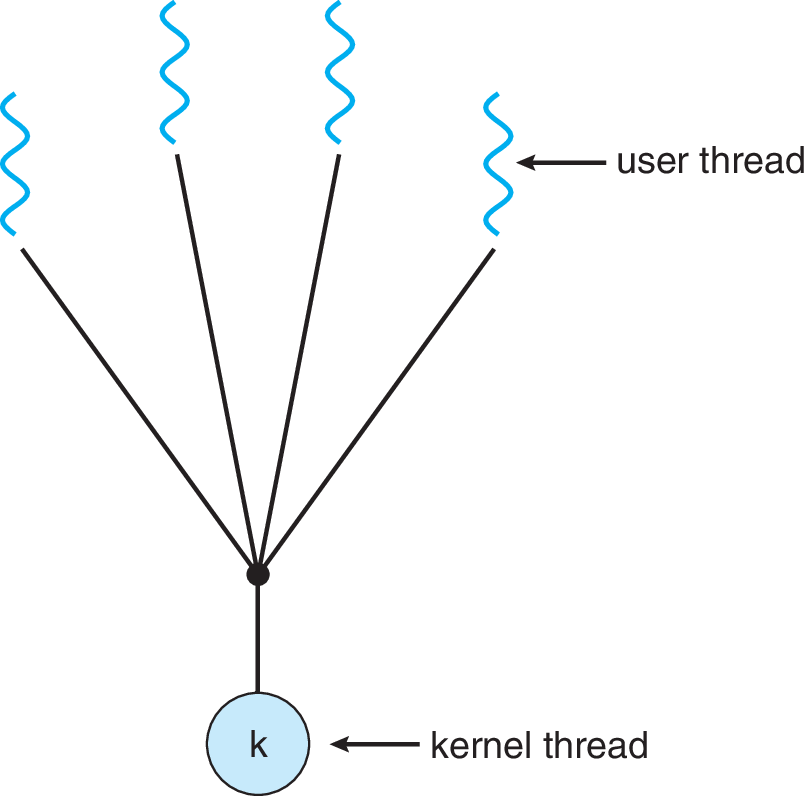
\includegraphics[width=4cm]{figs/01-4_05.pdf}
  \end{center}  

  Solaris: biblioteca {\em green threads}

  
\end{frame}

%---------------------------------------------------------------------
\begin{frame}
  \frametitle{ {\em One-to-one} }
  
  \begin{itemize}
    \item + {\em Threads} ejecutando {\em syscall} no bloquean el proceso
    \item + Asignables a distintos {\em core}s
    \item - Creación implica ejecutar {\em syscall}s
    \item - Sistemas Operativos limitan el máximo número de {\em threads}
  \end{itemize}

  \begin{center}
    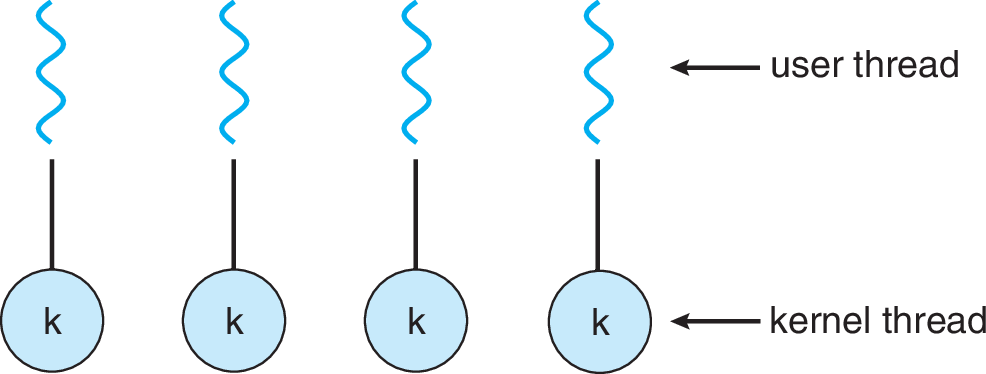
\includegraphics[width=6cm]{figs/01-4_06.pdf}
  \end{center}  

  Linux \& Windows
  
\end{frame}


%---------------------------------------------------------------------
\begin{frame}
  \frametitle{ {\em Many-to-many} }
  
  \begin{itemize}
    \item + Usuario pueden creer número ilimitado de {\em threads}
    \item + Asignación de {\em user thread} a {\em kernel thread} se hace {\em on-demand}
    \item + {\em Threads} ejecutando {\em syscall} no bloquean el proceso
    \item - Creación implica ejecutar {\em syscall}s
    \item - Sistemas Operativos limitan el máximo número de {\em threads}
  \end{itemize}

  \begin{center}
    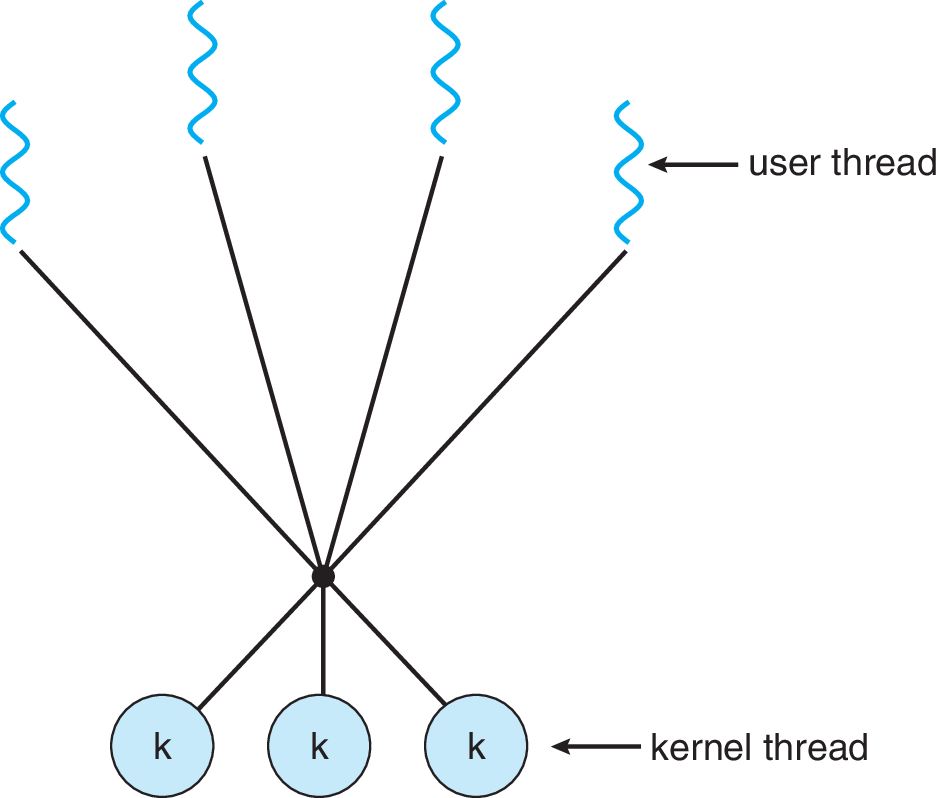
\includegraphics[width=4cm]{figs/01-4_07.pdf}
  \end{center}  

  %Linux \& Windows.
  
\end{frame}

%---------------------------------------------------------------------
\subsection{Bibliotecas de {\em thread}s}

\begin{frame}
  \frametitle{ Bibliotecas de {\em thread}s }

  Tres principales:
  
  \begin{itemize}
    \item POSIX Pthreads (kernel ó user)
    \item Windows Threads (kernel)
    \item Java threads (user)
  \end{itemize}


\end{frame}

%---------------------------------------------------------------------
\begin{frame}
  \frametitle{POSIX Pthreads}

  POSIX standard IEEE 1003.1c (especificación)
  
  API para creación y sincronización de {\em thread}s.
  
  Implementaciones para Linux, Mac OS X, Solaris
  
  \begin{itemize}
    \item {\tt pthread\_t}, identificador
    \item {\tt pthread\_create()}, creación de {\em thread}
    \item {\tt pthread\_join()}, padre espera que hijo(s) termine(n)
    \item {\tt pthread\_exit()}, termina el {\em thread} actual
  \end{itemize}
  
\end{frame}

%---------------------------------------------------------------------
\begin{frame}
  \frametitle{Windows Threads}

  Disponible nativamente en Windows API (kernel {\em thread}s)
    
  \begin{itemize}
    \item {\tt HANDLE}, permite acceder al {\em thread} (puntero)
    \item {\tt CreateThread()}, creación de {\em thread}
    \item {\tt WaitForSingleObject()} padre espera que hijo termine
    \item {\tt WaitForMultipleObjects()} padre espera que hijo(s) termine(n)
    \item {\tt CloseHandle()}, borra el {\em thread} indicado
  \end{itemize}
  
\end{frame}

%---------------------------------------------------------------------
\begin{frame}
  \frametitle{Java Threads}

  Implementado como biblioteca nativa en la JVM
  
  Se consideran {\em user thread}s ya que la JVM ejecuta sobre algún Sistema Operativo {\em host}
    
  \begin{itemize}
    \item Creación: extender clase {\tt Thread} y hacer {\em override} del método {\tt run()}
    \item Creación: clase que implementa la interfaz {\tt Runnable}
    \item {\em Thread} es efectivamente creado al invocar {\tt start()}
      \begin{enumerate}
        \item Asigna memoria para el nuevo objeto {\em thread} en la JVM
        \item Llama al método {\tt run()} iniciando la ejecución del {\em thread}
      \end{enumerate}
    \item Esperar que un {\em thread} hijo termine: {\tt join()}
  \end{itemize}
  
\end{frame}

%---------------------------------------------------------------------
\begin{frame}[fragile]
  \frametitle{{\em Multithreading} implícito}

  Usar eficientemente {\em thread}s no es fácil.
  
  ¿Y si le dejamos el trabajo al compilador o bibliotecas?
  
  \begin{itemize}
    \item {\em Thread-pools}: piscinas de {\em threads} disponibles
      \begin{itemize}
        \item Windows API: {\tt QueueUserWorkItem( \&PoolFunction,...)}
        \item Java: package {\tt java.util.concurrent}
      \end{itemize}
    \item {\tt OpenMP}: directivas para identificar regiones paralelas
      \begin{itemize}
        \item Popular en C, C++, FORTRAN
        \item Número de {\em threads} elegidos dinámicamente (p.ej: $\#$cores)
      \end{itemize}
    \item {\tt Grand Central Dispatch}
      \begin{itemize}
        \item Extensiones para C, C++
        \item Usado en Mac OS X, y en iOS
        \item Bloques de paralelismo: \verb+^{ printf("parallel");}+
      \end{itemize}
  \end{itemize}

\end{frame}

%---------------------------------------------------------------------
\begin{frame}
  \frametitle{Semántica de {\tt fork}/{\tt exec} y señales}
  
  Aún quedan algunas situaciones ``poco claras''
  
  \begin{itemize}
    \item Semántica de {\tt fork()} y {\tt exec()} en proceso {\em multithreaded}
      \begin{itemize}
        \item ¿Se duplican todos los {\em thread}s o solo el actual?
        \item ¿{\tt exec()} reemplaza todos los {\em thread}s?
      \end{itemize}
    \item Semántica de señales ({\em signal}s) en Unix, ¿quién la recibe?
      \begin{itemize}
        \item Un {\em thread}, aquél al cual se le aplica
        \item A todos los {\em thread}s del proceso
        \item A algunos {\em thread}s
        \item Siempre al mismo {\em thread}
      \end{itemize}
  \end{itemize}

\end{frame}

%---------------------------------------------------------------------
\begin{frame}
  \frametitle{Resumen: {\em Threads}}
  \framesubtitle{Algunos puntos clave}
  
  \begin{itemize}
    \item {\em Thread}: flujo de control básico dentro de un proceso
    \item Múltiples {\em thread}s en el mismo proceso comparten espacio de memoria
    \item {\em User thread}s: fáciles de crear, pero no visto por el Sistema Operativo
    \item {\em Kernel thread}s: manejables por el Sistema Operativo, más costosos de crear
    \item MacOSX, Windows, Linux, soportan {\em kernel thread}s y hacen {\em mapping} a {\em user thread}s
    \item Bibliotecas de {\em thread}s más comunes: Pthreads, Windows threads, Java threads
  \end{itemize}

\end{frame}
%---------------------------------------------------------------------
\section{Planificación de CPU}


%---------------------------------------------------------------------
\begin{frame}
  \frametitle{Planificación $\equiv$ {\em Scheduling}}

  {\bf ¡Multiprogramación y Time-sharing ({\em multitasking})!}
  
  \onslide<2->{
  \begin{block}{Objetivo de tener multiprogramación}
    {\bf Maximizar utilización de (una) CPU}
  \end{block}
  }

  \onslide<2->{
  \begin{block}{Objetivo de tener {\em multitasking}}
    {\bf Asignar tiempo de (una) CPU frecuentemente a todos los procesos}
  \end{block}
  }

%  ¿Qué queremos? \onslide<2->{{\bf ¡Multiprogramación y Time-sharing ({\em multitasking})!}}
%  
%  \onslide<3->{¿Cuándo lo queremos?} \onslide<4->{{\bf ASAP}\footnote{As Soon As Possible}}
%  
%  \onslide<5->{¿Cómo lo conseguimos?} \onslide<6->{Con {\bf ¡planificación ({\em scheduling})!}}
%
%  \onslide<7->{
%  \begin{block}{Objetivo de tener multiprogramación}
%    {\bf Maximizar utilización de (una) CPU}
%  \end{block}
%  }
%
%  \onslide<8->{
%  \begin{block}{Objetivo de tener {\em multitasking}}
%    {\bf Asignar tiempo de (una) CPU frecuentemente a todos los procesos}
%  \end{block}
%  }
%
%  \onslide<9->{Muchos procesos en estado {\em ready}}
%  
%  \onslide<10->{\ldots ¿qué hacer con ellos?}
%  
%  \begin{center}
%    \onslide<11->{{\bf ¡Colas!}}
%  \end{center}
  
\end{frame}


%---------------------------------------------------------------------
\begin{frame}
  \frametitle{Colas de {\em scheduling}}

  Múltiples colas
  
  \begin{center}
    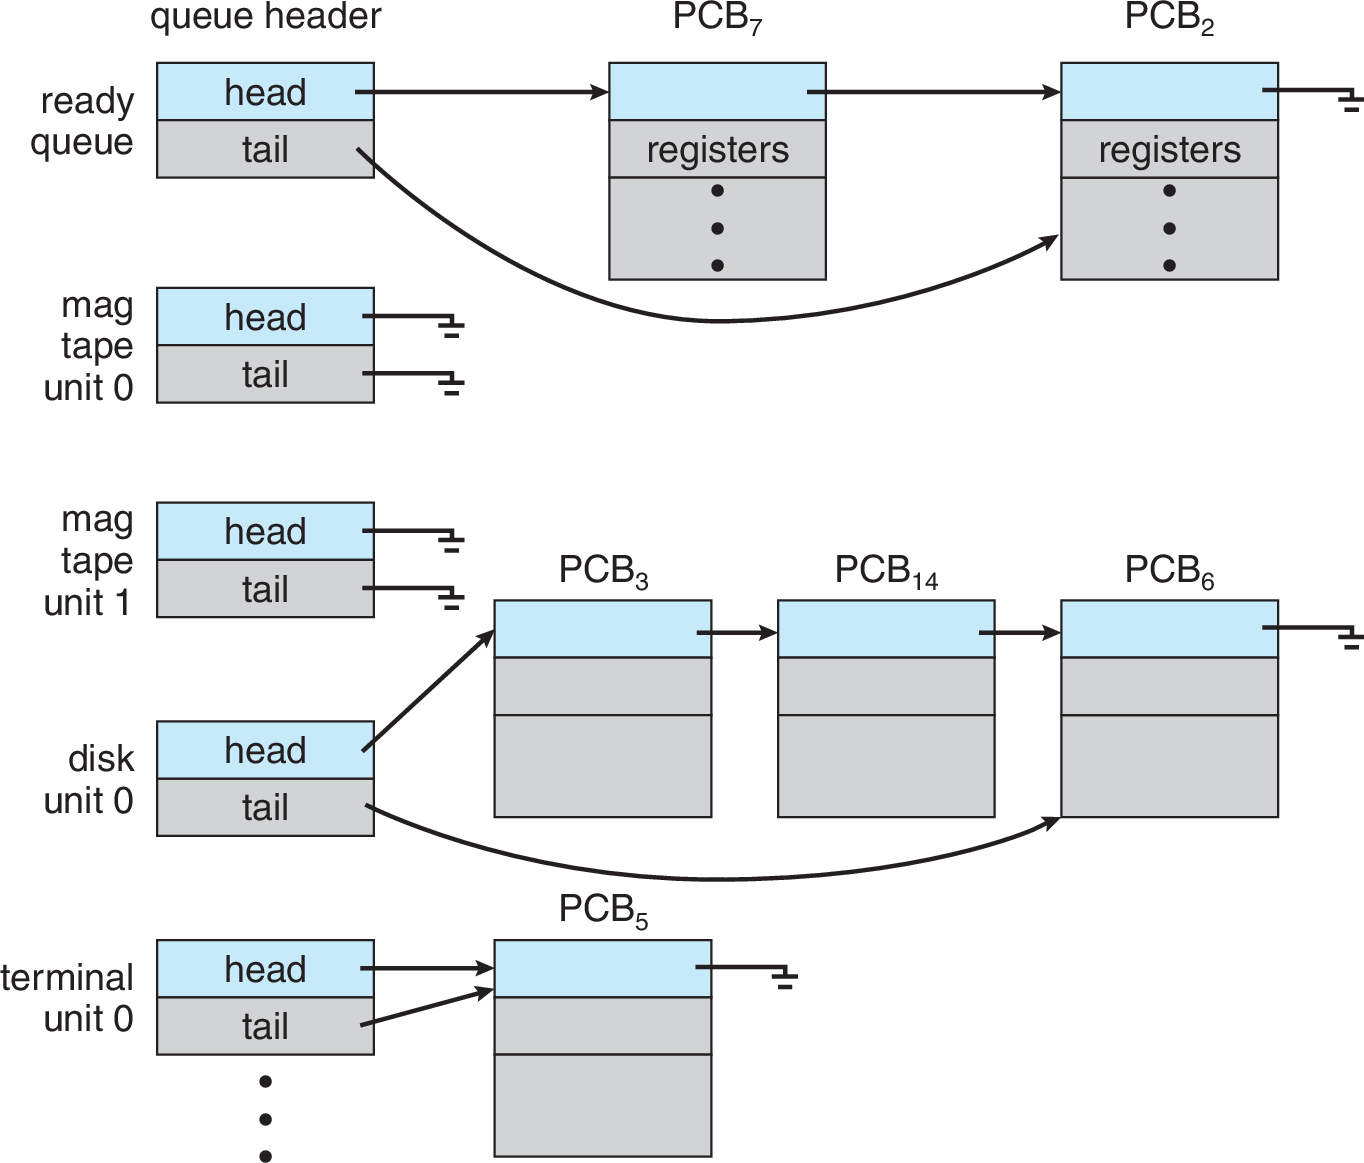
\includegraphics[width=8cm]{figs/01-3_05.pdf}
  \end{center}


\end{frame}

%---------------------------------------------------------------------
\begin{frame}
  \frametitle{Colas de {\em scheduling}}

  Planificación puede ser vista como un sistema de {\em manejo de colas}

  \onslide<2->{
  \begin{center}
    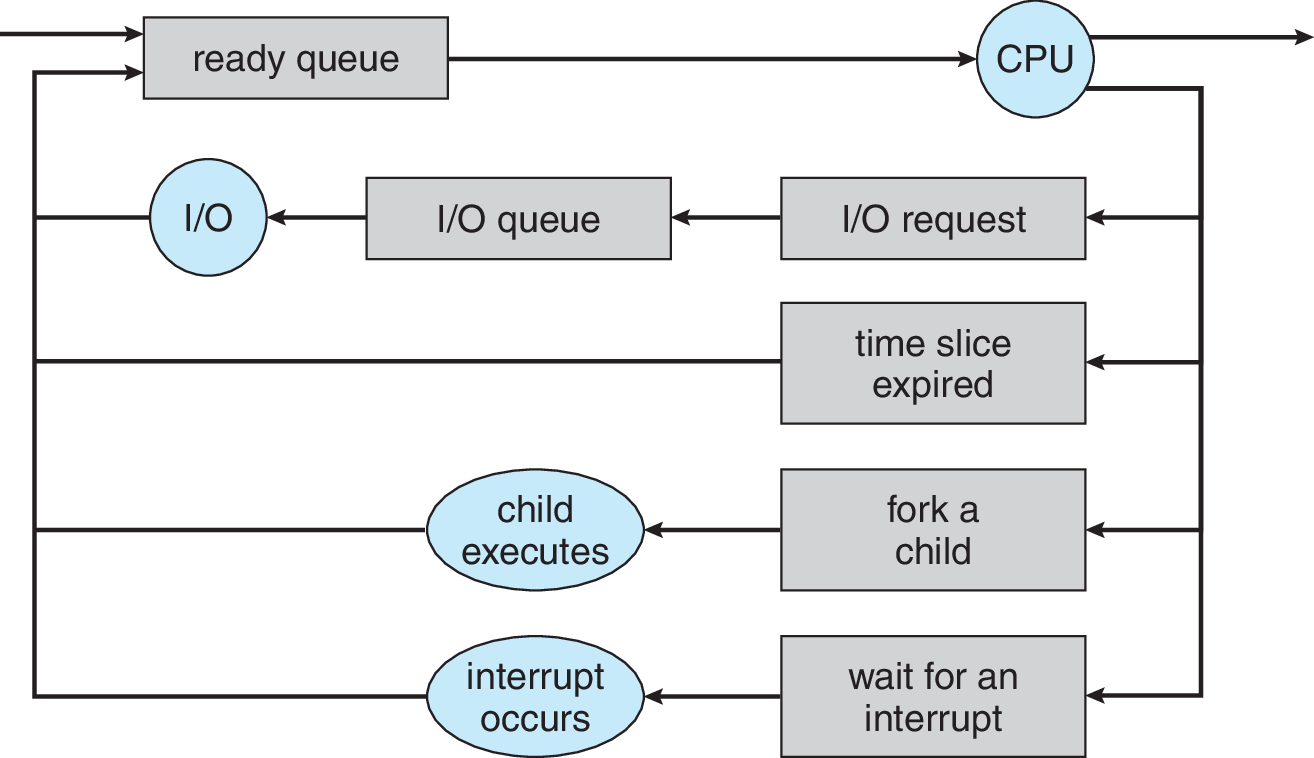
\includegraphics[width=8cm]{figs/01-3_06.pdf}
  \end{center}
  }
  
  \onslide<3->{¿Bajo qué criterio?}
  \onslide<4->{ $\longrightarrow$ {\bf algoritmos de {\em scheduling}}}


\end{frame}


%---------------------------------------------------------------------
\begin{frame}
  \frametitle{Distintos {\em schedulers} en un S.O.}

  \begin{description}
    \item[Long-term Scheduler]<2-> Determina qué procesos son admitidos en la {\em cola ready}.
                               Determina el {\bf grado de multiprogramación}.
    \item[Short-term Scheduler]<3-> Selecciona procesos {\em ready} de una o más colas para ejecutar.
    \item[Medium-term Scheduler]<4-> Modificación temporal del grado de multiprogramación, haciendo {\bf swapping}
  \end{description}
  
  \onslide<5->{
  \begin{center}
    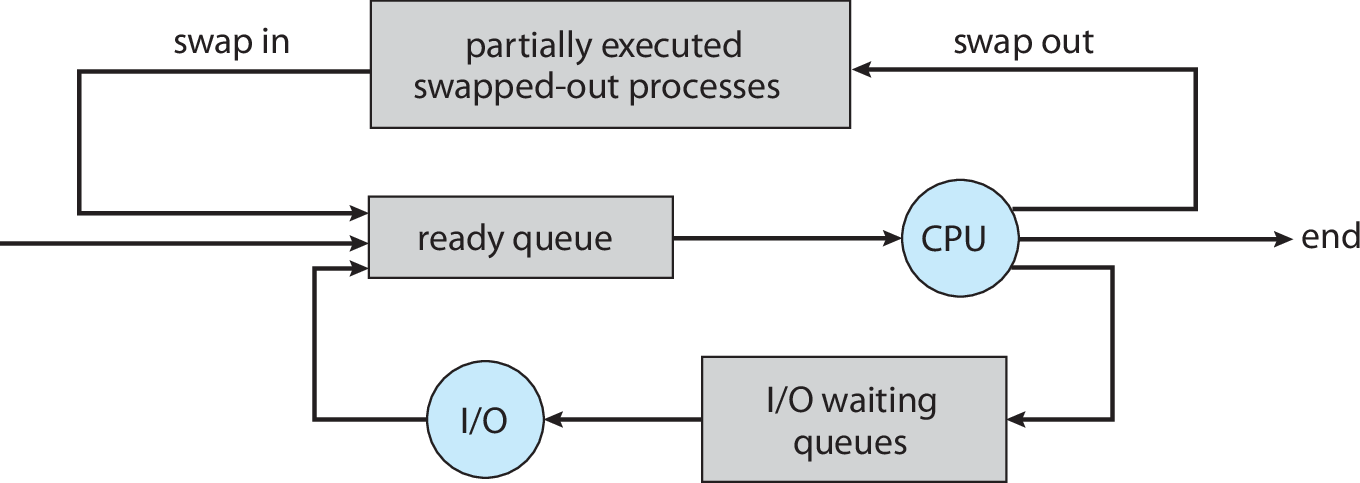
\includegraphics[width=8cm]{figs/01-3_07.pdf}
  \end{center}
  }  

\end{frame}

%---------------------------------------------------------------------
\begin{frame}
  \frametitle{¿Y si estamos siempre haciendo {\em Scheduling}?}
  \framesubtitle{i.e. ``exceso de burocracia''}

  {\em Scheduling} es importante para proveer {\bf multiprogramación}
  
  \onslide<2->{\ldots pero {\em scheduling} y {\em context switch} {\bf son sólo {\em overhead}}}
  
  \begin{itemize}
    \item<3-> ¿Qué pasa si el {\em scheduler} demora más tiempo de lo que toma el proceso?
    \item<4-> ¿Qué pasa si el {\em context switch} demora más tiempo de lo que toma el proceso?
    \item<5-> ¿Qué pasa si se le asigna poco tiempo a cada proceso?
    \item<6-> ¿Qué pasa si hay muchos procesos {\em ready}?
  \end{itemize}
  
  \onslide<7->{
  \begin{block}{}
    Contención de procesos se refleja en {\bf thrashing}   
  \end{block}
  }
  
  \onslide<8->{¿Los SS.OO. móviles permiten {\em multitasking}?}
  \begin{itemize}
    \item <9->{Hasta iOS 4, no había {\em multitasking} para procesos de usuasrio.}
    \item <10->{Android usa {\em servicios}: {\em multitasking} para procesos de sistema, que ejecutan tareas en el {\em background}}
  \end{itemize}
  
\end{frame}

%---------------------------------------------------------------------

%\begin{frame}
%  \frametitle{Planificación de CPU}
%
%  {\bf ¡Multiprogramación y Time-sharing ({\em multitasking})!}
%  
%  \onslide<2->{
%  \begin{block}{Objetivo de tener multiprogramación}
%    {\bf Maximizar utilización de (una) CPU}
%  \end{block}
%  }
%
%  \onslide<2->{
%  \begin{block}{Objetivo de tener {\em multitasking}}
%    {\bf Asignar tiempo de (una) CPU frecuentemente a todos los procesos}
%  \end{block}
%  }
%
%\end{frame}

%---------------------------------------------------------------------
%\begin{frame}
%  \frametitle{Colas de {\em scheduling}}
%
%  Planificación puede ser vista como un sistema de {\em manejo de colas}
%
%  \onslide<2->{
%  \begin{center}
%    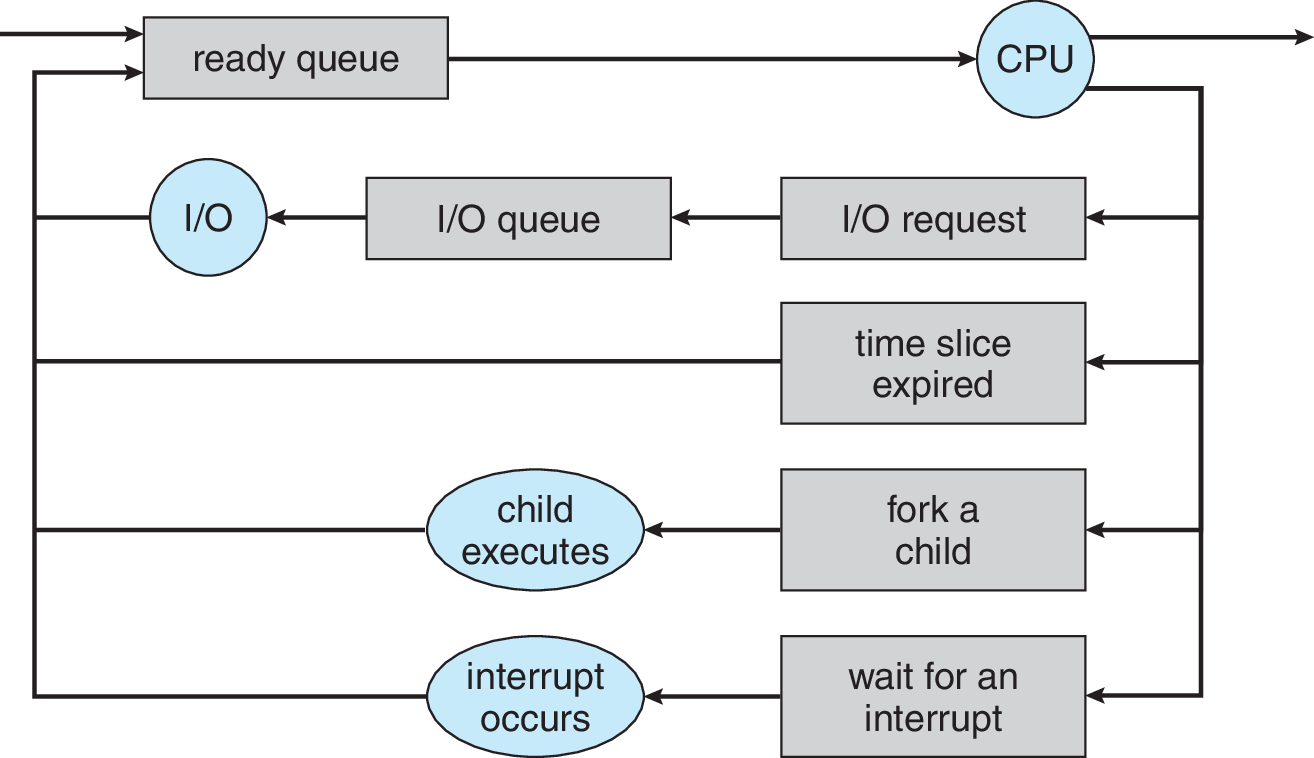
\includegraphics[width=8cm]{figs/01-3_06.pdf}
%  \end{center}
%  }
%  
%  \onslide<3->{¿Bajo qué criterio?}
%  \onslide<3->{ $\longrightarrow$ {\bf algoritmos de {\em scheduling}}}
%
%\end{frame}


%---------------------------------------------------------------------
\begin{frame}
  \frametitle{Ejecución típica de un proceso}

  \begin{columns}
  \begin{column}[T]{8cm}
    Un proceso pasa por dos etapas
    \begin{itemize}
      \item Uso de CPU (CPU-burst)
      \item Espera por E/S (I/O-burst)
    \end{itemize}
    Procesos suelen estar dominados por uno u otro
    \begin{itemize}
      \item CPU-bound
      \item I/O-bound
    \end{itemize}
  \end{column}  
  \begin{column}[T]{4cm}
    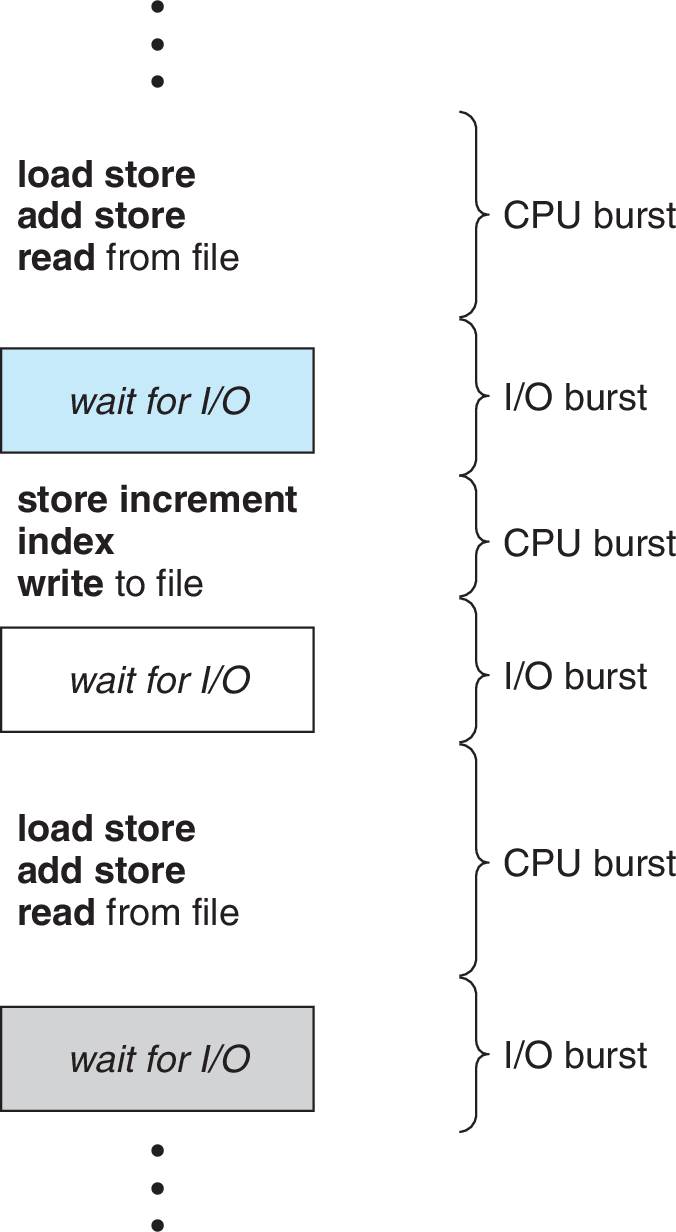
\includegraphics[width=4cm]{figs/01-6_01.pdf}
  \end{column}
  \end{columns}

\end{frame}

%---------------------------------------------------------------------
\begin{frame}
  \frametitle{Ejecución típica de un proceso}
  \framesubtitle{Duración de CPU-burst}
  
  ¿Cuánto dura típicamente un CPU-burst?
  
  No hay una respuesta única, pero \ldots
  
  \begin{center}
    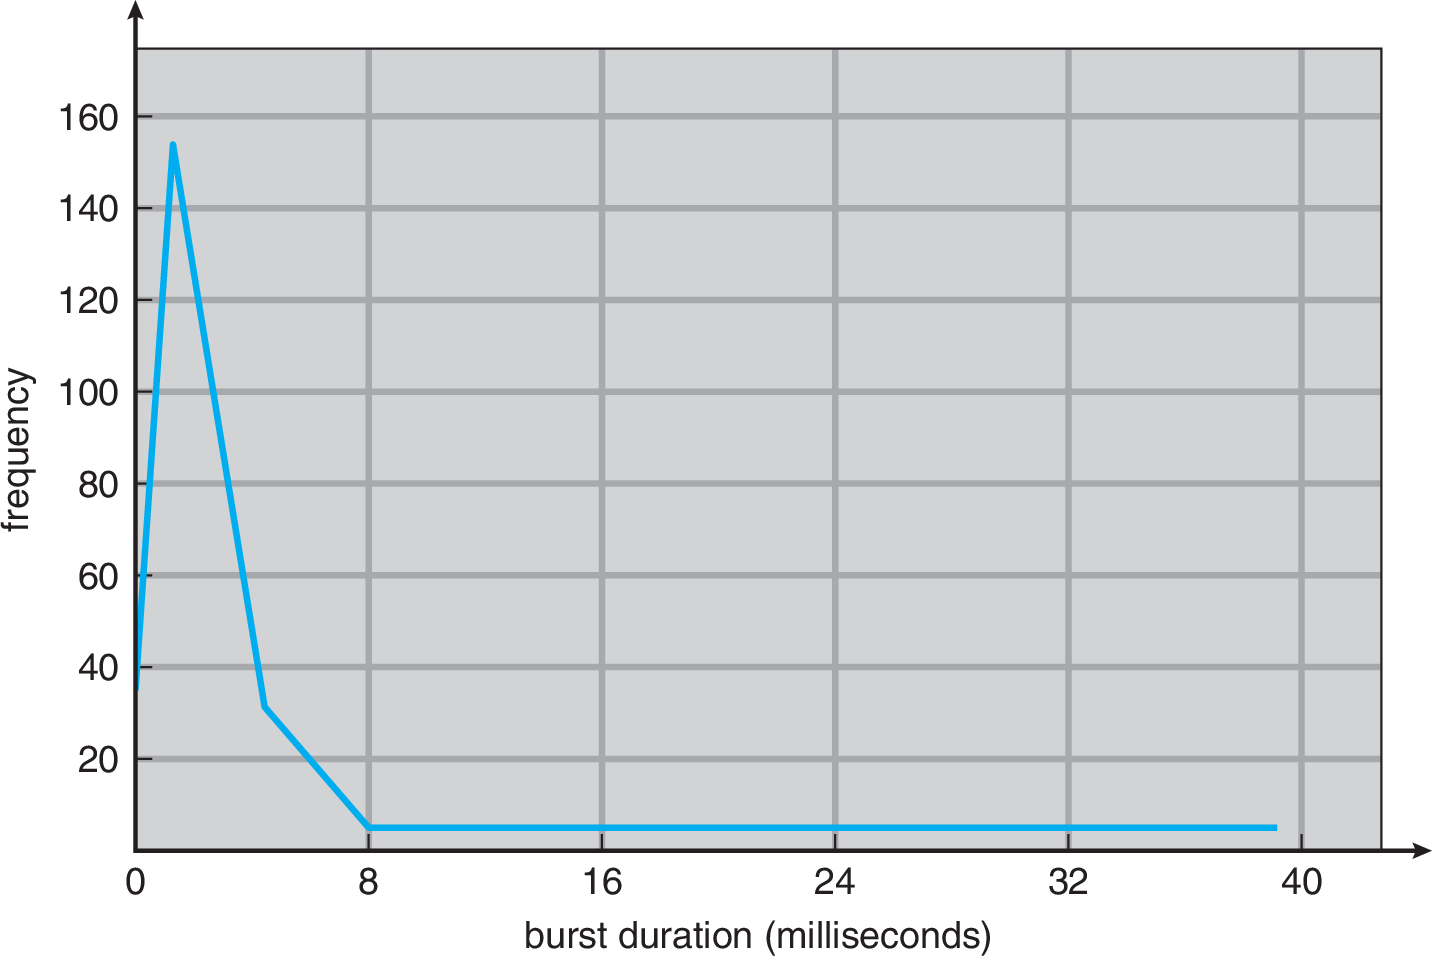
\includegraphics[width=8cm]{figs/01-6_02.pdf}
  \end{center}
  
  Duración de CPU-burst podría afectar el algoritmo de {\em scheduling}

\end{frame}

%---------------------------------------------------------------------
\begin{frame}
  \frametitle{{\em Tipos de {\em scheduling}}}

  Hay que tomar decisión de {\em scheduling} cuando:
  \begin{itemize}
    \item<2->(a) Proceso pasa de {\bf Running} a {\bf Waiting}
    \item<2->(b) Proceso pasa de {\bf Running} a {\bf Ready}
    \item<2->(c) Proceso pasa de {\bf Waiting} a {\bf Ready}
    \item<2->(d) Proceso termina
  \end{itemize}
  
  \onslide<3->{
  Dos tipos de {\em scheduling}
  
  \begin{block}{{\em Scheduling} con expropiación ({\bf preemptive})}
    Requiere interrupciones por {\em timer}
    
    Requiere cuidados de sincronización
  \end{block}

  \begin{block}{{\em Scheduling} sin expropiación ({\bf non-preemptive})}
    Sólo en (a) y (d). Proceso sólo libera la CPU voluntariamente.
    
    Windows 3.1, MacOS (antes de X). También se conoce como {\em scheduling cooperativo}
    
  \end{block}
  }

\end{frame}
%---------------------------------------------------------------------
\begin{frame}
  \frametitle{Criterios de {\em scheduling}}

  ¿Qué algoritmo puede ser mejor? \onslide<2->{\ldots depende}
  
  \begin{description}
     \item<3->[Uso de CPU] Mantener la CPU lo más usada posible
     \item<3->[Throughput] Cantidad procesos atendidos por unidad de tiempo
     \item<3->[Turnaround time] Tiempo total de un proceso, incluyendo esperas (wall-clock time)
     \item<3->[Waiting time] Tiempo de espera de un proceso en estado {\bf Ready}
     \item<3->[Response time] Importante para sistemas interactivos
  \end{description}
  
  \onslide<4->{¿Qué tiempo es mejor minimizar? ...}
  
  \onslide<4->{¿Tiempo promedio? ¿Tiempo máximo? ¿Varianza?}

\end{frame}
%---------------------------------------------------------------------
\begin{frame}
  \frametitle{{\em First-Come First-Served} (FCFS)}
  \framesubtitle{Por orden de llegada}
  
  El más simple: una cola FIFO

  Ejemplo: Procesos en cola: $P=\{P_1,P_2,P_3\}$, con tiempos de ejecución ({\em burst-time})
           $T=\{T_1=24,T_2=3,T_3=3\}$ en milisegundos
           
  \begin{itemize}
    \item Tiempo promedio de espera, para el orden $P_1, P_2, P_3$ \onslide<2->{$\to 17$ms}
    \item Tiempo promedio de espera, para el orden $P_2, P_3, P_1$ \onslide<2->{$\to 3$ms}
  \end{itemize}

  \onslide<3->{Non-preemptive}  
  \begin{itemize}
    \item<4-> +Simple
    \item<4-> -Poco predecible. Procesos CPU-bound pueden bloquear a los I/O-bound,
           bajo una secuencia ``desafortunada'' de llegada
  \end{itemize}

\end{frame}

%---------------------------------------------------------------------
\begin{frame}
  \frametitle{{\em Shortest-Job First} (SJF)}
  \framesubtitle{El más corto primero}

  Ejemplo: Procesos en cola: $P=\{P_1,P_2,P_3,P_4\}$, 
           $T=\{T_1=6,T_2=8,T_3=7,T_4=3\}$

  \begin{itemize}
    \item Tiempo promedio de espera: \onslide<2->{$\to 7$ms}
    \item<3->Con FCFS: \onslide<4->{$\to 10.25$ms}
  \end{itemize}

  \begin{itemize}
    \item<4-> +¡Óptimo! en tiempo de espera promedio (demostrable)
    \item<4-> -¿Cómo saber cuánto se tomará cada proceso?
%      \begin{itemize}
%        \item En {\em long-term scheduling} usuarios pueden especificar tiempo máximo 
%        \item En {\em short-term scheduling} hay que aproximarlo
%      \end{itemize}
  \end{itemize}

\end{frame}

%---------------------------------------------------------------------
\begin{frame}
  \frametitle{{\em Shortest-Job First} (SJF)}
  \framesubtitle{El pronóstico del tiempo}
  
  Supuesto: el próximo {\em burst} durará lo mismo que el anterior
  
  \onslide<2->{Método de aproximación: {\bf promedio exponencial} ({\em exponential average})
               sobre los {\em burst} anteriores}
               
  \onslide<3->{
  Sea $t_n$ el tiempo que tomó el $n$-ésimo {\em burst}, y $\tau_{n+1}$ el valor predicho.
  Se define, con $0 \leq \alpha \leq 1$:
  \[ \tau_{n+1} = \alpha t_n + (1-\alpha)\tau_n \]
  }
  
  \onslide<4->{
  $\alpha$ determina ``el peso de la historia'':
    \begin{itemize}
      \item $\alpha=0 \Rightarrow \tau_{n+1} = \tau_n$
      \item $\alpha=1 \Rightarrow \tau_{n+1} = t_n$
    \end{itemize}
  }
  
  \onslide<5->{
  Expansión:
  \[ \tau_{n+1} = \alpha t_n + (1-\alpha)\alpha t_{n-1} + \ldots + (1-\alpha)^j \alpha t_{n-j} + \ldots (1-\alpha)^{n+1}\tau_0 \]
  }

\end{frame}

%---------------------------------------------------------------------
\begin{frame}
  \frametitle{{\em Shortest-Job First} (SJF)}
  \framesubtitle{El pronóstico del tiempo}

  $\alpha = 1/2, \tau_0=10$
  
  \begin{center}
    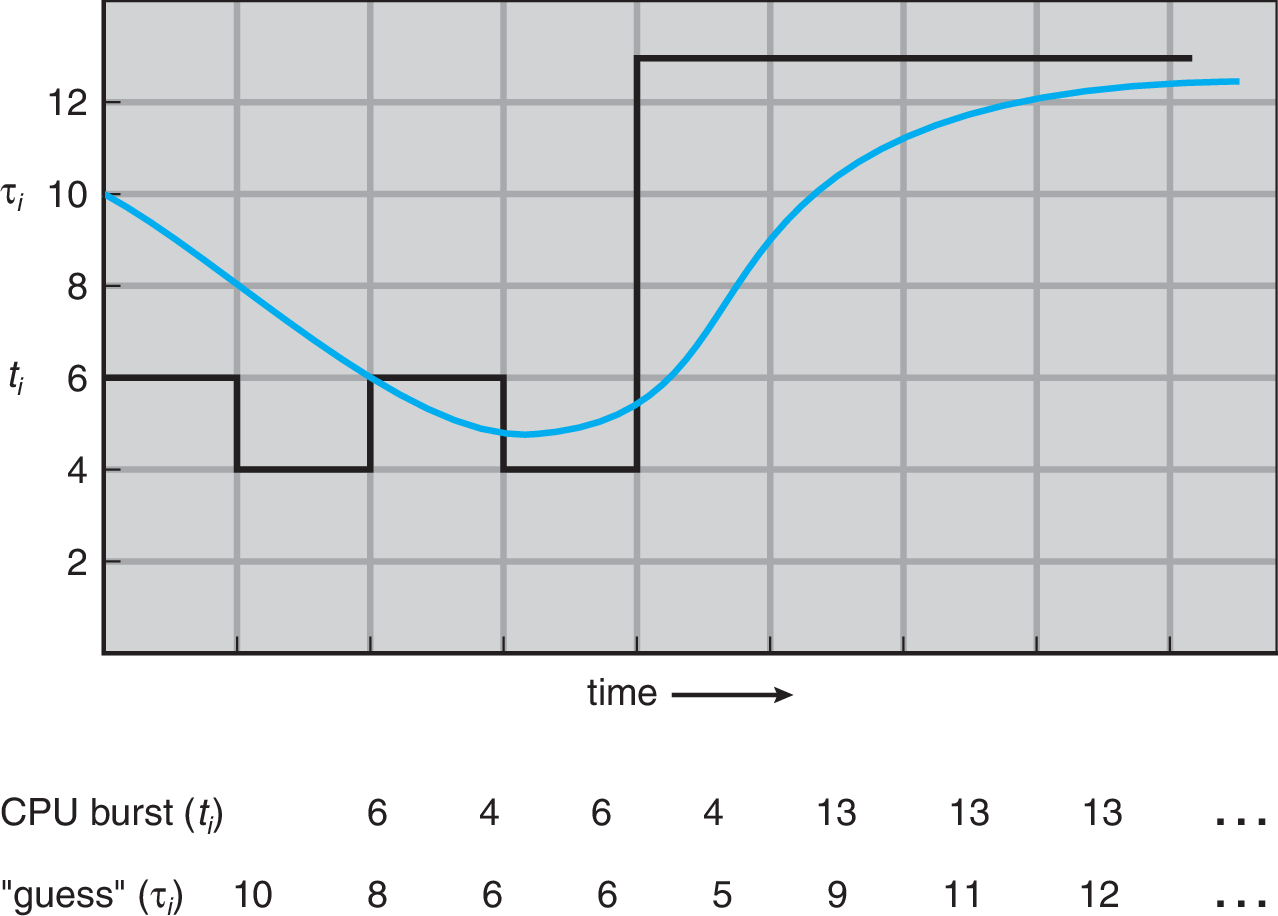
\includegraphics[width=8cm]{figs/01-6_03.pdf}
  \end{center}



\end{frame}

%---------------------------------------------------------------------
\begin{frame}
  \frametitle{{\em Shortest-Job First} (SJF)}
  \framesubtitle{Versión {\em preemptive}}

  ¿Qué hacer cuando llega un proceso nuevo?
  
  \onslide<2->{
  Decidir en base al {\bf tiempo restante}
  
  Ejemplo: $P=\{P_1,P_2,P_3,P_4\}$,
           tiempos de llegada $\{0,1,2,3\}$
           $T=\{8,4,9,5\}$  
  }
  
  \onslide<3->{
  \begin{itemize}
    \item Ejecución {\em preemptive}: \onslide<4->{$\to 6.5$ms} 
    \item Ejecución {\em non-preemptive}: \onslide<5->{$\to 7.75$ms}
  \end{itemize}
  }
  
\end{frame}

%---------------------------------------------------------------------
\begin{frame}
  \frametitle{{\em Scheduling} con prioridades}
%  \framesubtitle{}

  Cada proceso tiene asociada una {\bf prioridad}
  
  \begin{itemize}
    \item Se atienden por orden de {\bf prioridad}
    \item Prioridades iguales: FCFS
    \item SJF es un {\em caso particular} de este algoritmo (¿por qué?)
    \item Muchos criterios para definir prioridades
  \end{itemize}
  
  \onslide<2->{Puede ser {\em non-preemptive} o {\em preemptive} (si llega uno con mayor prioridad,
               ejecuta de inmediato)}
  
  \onslide<3->{
  \begin{itemize}
    \item -Inanición de los que tengan baja prioridad
  \end{itemize}
  }

\end{frame}
%---------------------------------------------------------------------
\begin{frame}
  \frametitle{{\em Round-Robin} (RR)}
%  \framesubtitle{}

  Ideal para {\em time-sharing}
  
  \onslide<2->{
  FCFS + Preemption + 
  {\em time quantum} o {\em time slice} $q$: unidad de tiempo\footnote{Típicamente $10$ a $100$ms}
  Cada proceso recibe un $q$ms para ejecutar.
  }
  
  \onslide<3->{
    Ejemplo: $P=\{P_1,P_2,P_3\}$,
           $T=\{24,3,3\}$  
  
  \begin{itemize}
    \item Tiempo de espera promedio: $\to 5.66$ms
  \end{itemize}
  }
  
  \onslide<4->{
  \begin{itemize}
    \item +Cada proceso recibe $1/n$ de CPU, para $n$ procesos
    \item +Ningún proceso espera más de $(n-1)\times q$ para ejecutar
    \item Altamente dependiente de la elección de $q$ (puede degenerar a FCFS)
  \end{itemize}
  }
  
\end{frame}

%---------------------------------------------------------------------
\begin{frame}
  \frametitle{Colas Multinivel}

  Múltiples colas, divididas por tipo de proceso.
  
  \begin{center}
    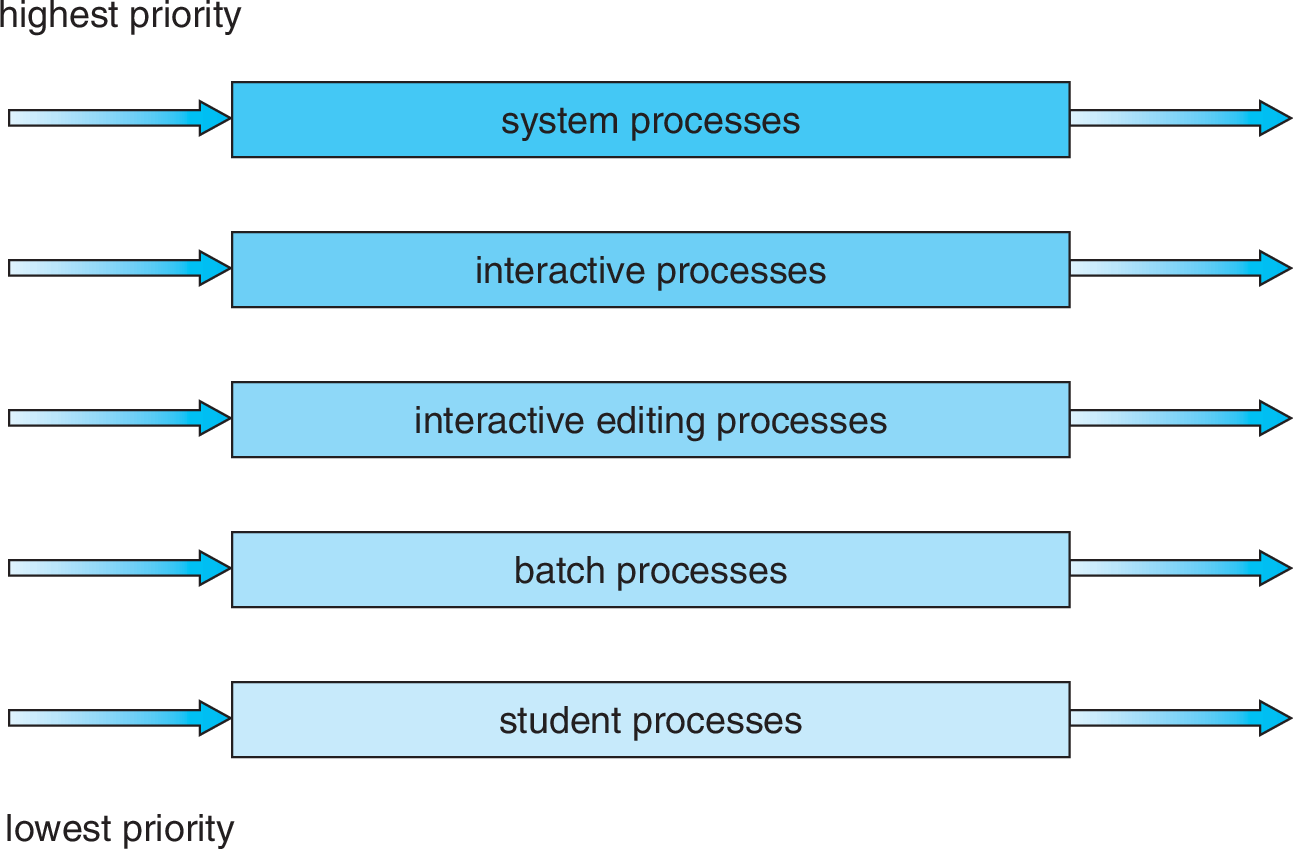
\includegraphics[width=7cm]{figs/01-6_06.pdf}
  \end{center}
  
  Varias alternativas:
  \begin{itemize}
    \item Prioridades entre colas, FCFS dentro de cada cola
    \item RR entre colas, con quántums diferenciados
  \end{itemize}

\end{frame}
%---------------------------------------------------------------------
\begin{frame}
  \frametitle{Colas Multinivel con Feedback (MLFQ)}

  Colas multinivel es muy rígido: procesos no cambian de cola

  \begin{center}
    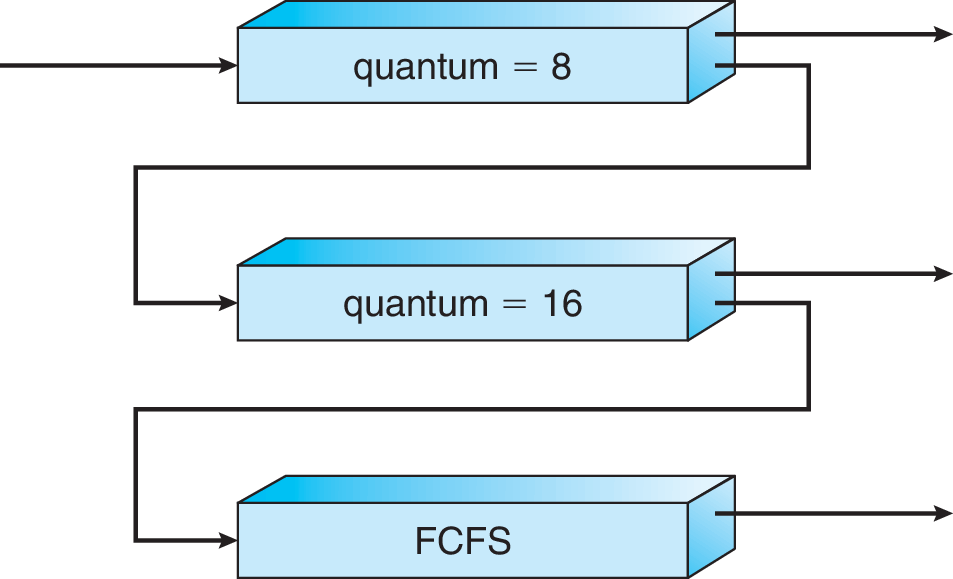
\includegraphics[width=5cm]{figs/01-6_07.pdf}
  \end{center}
  
  \begin{itemize}
    \item Colas con quántum diferenciado. 
    \item Proceso que no terminan en su quántum pasan a cola inferior
    \item Proceso que entregan la CPU permanecen la misma cola
    \item Dentro de cada cola, {\em scheduling} es FCFS
    \item Favorece procesos con CPU {\em burst} cortos
    \item Eventualmente se puede promover de nivel a los que han esperado más
  \end{itemize}

\end{frame}
%---------------------------------------------------------------------
\begin{frame}
  \frametitle{{\em Scheduling} en multi-procesador}

  Para un procesador no hay una mejor solución \ldots 
  \onslide<2->{para múltiples procesadores es más difícil}
  
  \begin{itemize}
    \item<3-> Modo asimétrico: distintos tipos de procesos a distintos cores
    \item<4-> Modo simétrico (SMP). Ampliamente soportado: Windows, Linux, MacOSX
      \begin{itemize}
        \item ¿colas por procesador o cola única?
        \item evitar que dos procesadores ejecuten el mismo proceso
      \end{itemize}
  \end{itemize}
    

\end{frame}
%---------------------------------------------------------------------
\begin{frame}
  \frametitle{{\em Scheduling} en multi-procesador}

  \begin{block}{{\bf Processor Affinity} (afinidad)}
  Considera efectos de {\em cache}

  \onslide<2->{Es más conveniente que un proceso se mantenga en el mismo procesador}
  
  \end{block}

  \onslide<3->{
  \begin{block}{{\bf Load Balancing} (balance de carga)}
  Objetivo: mantener carga similar entre procesadores
  
  \onslide<4->{Si hay procesadores desocupados, algunos
  procesos son migrados a ellos. Modo {\em push} ó {\em pull}}
    
  \end{block}
  }
  
  \onslide<5->{¿Objetivos conflictivos?}
\end{frame}

%---------------------------------------------------------------------
\begin{frame}
  \frametitle{{\em Scheduling} en Windows}

  \begin{itemize}
    \item 3.1, 95, 98. Preemptive para 32-bit. Cooperative para 16-bit.
    \item NT-based. MLFQ con 32 prioridades.
      \begin{itemize}
        \item 16 prioridades normales
        \item 16 prioridades {\em Real-Time}
        \item S.O. puede modificar prioridad para mejorar interactividad
      \end{itemize}
  \end{itemize}
\end{frame}

%---------------------------------------------------------------------
\begin{frame}
  \frametitle{{\em Scheduling} en MacOS}

  \begin{itemize}
    \item Hasta MacOS 9: cooperativo. RR entre procesos.
    \item MacOSX: MLFQ con 4 prioridades
      \begin{itemize}
        \item Normal
        \item System high-priority
        \item Kernel mode only
        \item Real-time
      \end{itemize}
  \end{itemize}

\end{frame}

%---------------------------------------------------------------------
\begin{frame}
  \frametitle{{\em Scheduling} en Linux}

  \begin{itemize}
    \item Linux 2.4. $O(n)$ {\em scheduler}. MLFQ. {\em Quantum}s no usados por completo se agregan a la siguiente ronda.
    \item Linux 2.6.0 a 2.6.22. $O(1)$ {\em scheduler}. Mejor soporte para SMP, mal soporte para tareas interactivas.
       \begin{itemize}
         \item Tiempo de selección independiente del número de procesos
       \end{itemize}
    \item Linux 2.6.23. {\em Completely Fair Scheduler} (CFS).
  \end{itemize}

\end{frame}
%---------------------------------------------------------------------
\begin{frame}
  \frametitle{Resumen: {\em Scheduling}}
  \frametitle{Algunos puntos importantes}
  
  \begin{itemize}
    \item {\em Scheduler} permite seleccionar el próximo proceso del conjunto {\em ready}
    \item Debe ser una decisión rápida
    \item Diferentes métricas para comparar algoritmos de {\em scheduling}
    \item Algoritmos clásicos:
      \begin{itemize}
        \item FCFS: simple, tiempo de espera impredecible
        \item SJF: óptimo en tiempo de espera, difícil de predecir
        \item RR: mejor para {\em time-sharing}, depende de $q$
        \item Prioridades: con expropiación, apropiado para {\em real-time}
        \item Multicolas, MLFQ: flexible y base para {\em schedulers} reales
      \end{itemize}  
    \item {\em Scheduling} para multiprocesadores
      \begin{itemize}
        \item Arquitecturas SMP requiere {\em tradeoff} entre afinidad y balance de carga
      \end{itemize}
  \end{itemize}

\end{frame}
%---------------------------------------------------------------------
\section{Sincronización de Procesos}

\begin{frame}
  \frametitle{Sincronización de Procesos}

  Cosas buenas:
  \begin{itemize}
    \item Tener {\em concurrencia} y {\em paralelismo}
    \item Crear {\em threads} livianos sobre el mismo espacio de memoria (no necesita {\em syscall} de {\em shared memory}) 
  \end{itemize}
  Pero \ldots
  \begin{itemize}
    \item Hay que coordinarlos (¿por qué?)
  \end{itemize}
  
\end{frame}

%---------------------------------------------------------------------
\begin{frame}[fragile]
  \frametitle{Regreso al Productor/Consumidor}
  Solución con {\em threads} productor y consumidor. 
  Variable {\tt counter} inicializada en {\tt 0} en memoria compartida.
  
\begin{minted}[mathescape,numbersep=5pt,gobble=2,frame=lines,framesep=2mm,fontsize=\scriptsize,linenos=true]{c}
  /** Productor **/
  while(true) {
    next_product = produce();
    while (counter == BUFFER_SIZE); /* do nothing */
    buffer[in] = next_product;
    in = (in+1)%BUFFER_SIZE;
    counter++;
  }
\end{minted}

\begin{minted}[mathescape,numbersep=5pt,gobble=2,frame=lines,framesep=2mm,fontsize=\scriptsize,linenos=true]{c}
  /** Consumidor **/  
  while(true) {
    while(counter == 0); /* do nothing */
    next_consumed = buffer[out];
    out = (out+1)%BUFFER_SIZE
    counter--;
    consume(next_consumed);
  }
\end{minted}  

\end{frame}

%---------------------------------------------------------------------
\begin{frame}[fragile]
  \frametitle{Regreso al Productor/Consumidor}

  ¿Qué podría salir mal?
  
  \onslide<2->{Supongamos {\tt counter=13}. Considere la secuencia:}
\begin{minted}[mathescape,numbersep=5pt,gobble=2,frame=lines,framesep=2mm,fontsize=\scriptsize]{c}
  counter++;  /** linea 7 productor **/
  counter--;  /** linea 6 consumidor **/
\end{minted}
  \onslide<3->{Resultado esperado: {\tt counter == 13}}
  
  \onslide<4->{Pero también podría ocurrir {\tt counter==12} o {\tt counter==14} (what?)}

\end{frame}

%---------------------------------------------------------------------
\begin{frame}[fragile]
  \frametitle{Regreso al Productor/Consumidor}
  \framesubtitle{Autoincremento en assembler o en bytecode}

  ¿Cómo se ejecutan los {\tt ++} y {\tt --} en hardware?

  Línea 7 productor: {\tt counter++}
\begin{minted}[mathescape,numbersep=5pt,gobble=2,frame=lines,framesep=2mm,fontsize=\scriptsize]{nasm}
  load r1, counter  ; copia del valor desde memoria a registro 1 
  inc r1            ; autoincremento de registros es comun en muchas arquitecturas 
  store counter, r1 ; guarda el valor de r1 en memoria 
\end{minted}

  Línea 6 consumidor: {\tt counter--}
\begin{minted}[mathescape,numbersep=5pt,gobble=2,frame=lines,framesep=2mm,fontsize=\scriptsize]{nasm}
  load r2, counter
  dec r2
  store counter, r2
\end{minted}

\end{frame}

%---------------------------------------------------------------------
\begin{frame}[fragile]
  \frametitle{Productor/Consumidor {\em multithreaded}}
  \framesubtitle{Because shit happens}
  
  Podría ocurrir este orden de ejecución (o talvez no)
  
  \begin{footnotesize}
  \begin{tabular}{llll}
  \onslide<2->{$t=0$ & productor  & {\tt load r1, counter}  & $r_1=13, r2=?, \mathit{counter}=13$ \\ \hline}
  \onslide<3->{$t=1$ & productor  & {\tt inc r1}            & $r_1=14, r2=?, \mathit{counter}=13$ \\ \hline}
  \onslide<4->{$t=2$ & consumidor & {\tt load r2, counter}  & $r_1=14, r2=13, \mathit{counter}=13$ \\ \hline}
  \onslide<5->{$t=3$ & consumidor & {\tt dec r2}            & $r_1=14, r2=12, \mathit{counter}=13$ \\ \hline}
  \onslide<6->{$t=4$ & productor &  {\tt store counter, r1} & $r_1=14, r2=12, \mathit{counter}=14$ \\ \hline}
  \onslide<7->{$t=5$ & consumidor & {\tt store counter, r2} & $r_1=14, r2=12, \mathit{counter}=12$ \\ }
  \end{tabular}
  \end{footnotesize}

  \onslide<8->{¿Podemos tener tan mala suerte para que ocurra así?}

  \onslide<9->{
  \begin{block}{{\bf Race condition} (condición de carrera o competencia)}
    Situación en que la salida de una operación depende del orden temporal de sus operaciones internas,
    el cual no está bajo control del programador.
  \end{block}
  }
\end{frame}

%---------------------------------------------------------------------
\begin{frame}
  \frametitle{Sincronización de {\em threads}}
  \framesubtitle{Un programador tenía un problema y decidió usar {\em threads}. tiene él problemas. Ahora dos }

  {\em Race conditions} hacen que el resultado de la ejecución no se pueda garantizar.
  \onslide<2->{
  \begin{alertblock}{{\bf Mala práctica}}
     El resultado de una ejecución puede depender de la entremezcla ({\em interleaving}) de la ejecución de sus {\em threads}  
  \end{alertblock}
  }
  
  \onslide<3->{
  \begin{exampleblock}{{\bf Buena práctica}}
    {\bf Evitar las race conditions}
  \end{exampleblock}
  }
  
  \onslide<3->{¿Como? Empleando métodos de {\bf sincronización} y {\bf coordinación}.}
   
\end{frame}
%---------------------------------------------------------------------
\subsection{El Problema de la Sección Crítica}

\begin{frame}
  \frametitle{El Problema de la Sección Crítica}

  Considere un sistema de $n$ procesos, $\{P_0,P_1,\ldots,P_{n-1}\}$.
  Cada proceso tiene un segmento de código llamado {\bf sección crítica}
  \begin{itemize}
    \item Dentro de su sección crítica el proceso puede modificar recursos compartidos
  \end{itemize}
  
  \onslide<2->{
  \begin{block}{Problema de la Sección Crítica}
    Diseñar un protocolo que no permita que dos procesos se encuentren en su sección crítica al mismo tiempo
  \end{block}
  }
  
  \begin{center}
    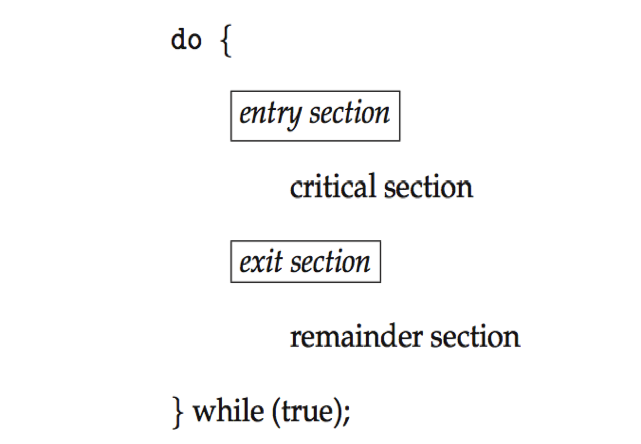
\includegraphics[width=5cm]{figs/01-seccioncritica.png}
  \end{center}
  
\end{frame}

%---------------------------------------------------------------------
\begin{frame}
  \frametitle{Requisitos para una solución}

  Una solución al problema de la sección crítica (SC) debe cumplir 3 requisitos:
  
  \begin{description}
    \item[{\bf Exclusión Mutua}] {\em A lo más uno}. Si $P_i$ se encuentra en su SC, entonces
                                 nadie más lo está.
    \item[{\bf Progreso}] {\em Al menos alguien puede entrar}. Si ningún proceso está en su SC, y hay
                          procesos que desean entrar, entonces los que quieren entrar deben ser capaces
                          de decidir quién entra, y decidirlo en un tiempo acotado.
    \item[{\bf Espera acotada}] {\em Ausencia de inanición}. Si un proceso quiere entrar a su SC, entonces
                                después de una cantidad limitada de turnos, el proceso podrá entrar.
                                Esto significa que nadie espera indefinidamente.
  \end{description}

\end{frame}

%---------------------------------------------------------------------
\subsection{Algunas soluciones al problema de la sección crítica}

\begin{frame}[fragile]
  \frametitle{Solución de Peterson}
  Solución para 2 procesos, propuesta por Gary L. Peterson, 1981.
  
  Variables compartidas: {\tt int turn; boolean flag[2];}

\begin{minted}[mathescape,numbersep=5pt,gobble=2,frame=lines,framesep=2mm,fontsize=\scriptsize,linenos=true]{c}
  /** Codigo para proceso P_i, i $\in$ {0,1}, j=1-i */
  
  do {
    flag[i] = true;
    turn = j;
    while(flag[j] && turn == j);
    
    /** SECCION CRITICA **/
    
    flag[i] = false;
    
    /** resto del codigo **/
  
  } while(true);

\end{minted}

\onslide<2->{¿En qué valor se inicializan {\tt turn} y {\tt flag}?}

\end{frame}

%---------------------------------------------------------------------
\begin{frame}
  \frametitle{Solución de Peterson}
  \framesubtitle{¿Cumple los requisitos?}
  
  {\bf Exclusión Mutua}
  
  \begin{itemize}
    \item $P_i$ puede entrar solamente si {\tt flag[j]==false} ó {\tt turn == i}
    \item Si $P_i$ y $P_j$ se encuentran ambos en la SC, entonces {\tt flag[0]==flag[1]==true}
    \item {\tt flag[0]==true} $\Rightarrow$ {\tt turn=i}
    \item {\tt flag[1]==true} $\Rightarrow$ {\tt turn=j}
    \item Pero {\tt i}$\neq${\tt j}, por lo tanto no pueden estar ambos en su SC
  \end{itemize}
  
\end{frame}

%---------------------------------------------------------------------
\begin{frame}
  \frametitle{Solución de Peterson}
  \framesubtitle{¿Cumple los requisitos?}

  {\bf Progreso}
  
  \begin{itemize}
    \item Si $P_i$ desea entrar a su SC, sólo puede estar detenido en la línea 6
    \item Entonces se cumple {\tt flag[j]==true} y {\tt turn==j}
    \item Si $P_j$ no desea entrar a su SC, entonces {\tt flag[j]==false}
    \item Si $P_j$ desea entrar, entonces {\tt turn==i} ó {\tt turn==j}
    \item En cualquier caso, uno de los que quiere entrar, entra 
  \end{itemize}

\end{frame}

%---------------------------------------------------------------------
\begin{frame}
  \frametitle{Solución de Peterson}
  \framesubtitle{¿Cumple los requisitos?}

  {\bf Espera acotada}
  
  \begin{itemize}
    \item Si $P_i$ desea entrar y está esperando, entonces {\tt flag[i]==true}, {\tt flag[j]==true} y {\tt turn==j}
    \item En cuanto $P_j$ sale, establece {\tt flag[j]=false}, y $P_i$ puede entrar (si empieza a ejecutar)
    \item Si $P_j$ intenta entrar inmediatamente, deberá establecer {\tt flag[j]=true} y {\tt turn=i}.
    \item Se cumple entonces {\tt flag[i]==true}, {\tt flag[j]==true}, y {\tt turn=i}, con lo que $P_j$ no puede entrar.    
    \item Por lo tanto después de, a lo más, 1 turno, $P_i$ puede entrar (espera acotada)
  \end{itemize}

\end{frame}

%---------------------------------------------------------------------
\begin{frame}[fragile]
  \frametitle{Sincronización por {\em hardware} }
  \framesubtitle{}

  Soluciones por {\em software} dependen de que existan {\bf instrucciones atómicas} por {\em hardware}:
  instrucciones {\bf ininterruptibles}

  Una solución más sencilla:
\begin{minted}[mathescape,numbersep=5pt,gobble=2,frame=lines,framesep=2mm,fontsize=\scriptsize,linenos=false]{c}
  /** Exclusion mutua **/
    do {
      lock = true;
      while (lock == false);
      
      /* SECCION CRITICA */
      
      lock = false;
  
      /* resto del codigo */
      
  }  while(true);
\end{minted}
  
  ¿Basta con esto?
\end{frame}


%---------------------------------------------------------------------
\begin{frame}[fragile]
  \frametitle{Sincronización por {\em hardware} }
  \framesubtitle{{\tt test\_and\_set()}}

  Algunas arquitecturas proveen instrucciones atómicas del tipo \verb+test_and_set+

\begin{minted}[mathescape,numbersep=5pt,gobble=2,frame=lines,framesep=2mm,fontsize=\scriptsize,linenos=false]{c}
  /** test_and_set() **/
    boolean test_and_set (boolean *target) {
      boolean rv = *target;
      *target = true;
  
      return rv;
    }
\end{minted}
  
\end{frame}

%---------------------------------------------------------------------
\begin{frame}[fragile]
  \frametitle{Sincronización por {\em hardware} }
  \framesubtitle{Exclusión mutua con {\tt test\_and\_set()}}

  ¿Cómo usarlo?

\begin{minted}[mathescape,numbersep=5pt,gobble=2,frame=lines,framesep=2mm,fontsize=\scriptsize,linenos=false]{c}
  /** Exclusion mutua usando test_and_set() **/
    do {
      while (test_and_set(&lock));
      
      /* SECCION CRITICA */
      
      lock = false;
  
      /* resto del codigo */
      
  }  while(true);
\end{minted}

\end{frame}

%---------------------------------------------------------------------
\begin{frame}[fragile]
  \frametitle{Sincronización por {\em hardware} }
  \framesubtitle{{\tt compare\_and\_swap()}}

  Otra instrucción atómica: \verb+compare_and_swap+

\begin{minted}[mathescape,numbersep=5pt,gobble=2,frame=lines,framesep=2mm,fontsize=\scriptsize,linenos=false]{c}
  /** compare_and_swap  **/
    boolean compare_and_swap (int *value, int expected, int new_value) {
      int temp = *value;

      if(*value == expected)
        *value = new_value;
  
      return temp;
    }
\end{minted}
  
\end{frame}

%---------------------------------------------------------------------
\begin{frame}[fragile]
  \frametitle{Sincronización por {\em hardware} }
  \framesubtitle{Exclusión mutua con {\tt compare\_and\_swap()}}

  ¿Cómo usarlo?

\begin{minted}[mathescape,numbersep=5pt,gobble=2,frame=lines,framesep=2mm,fontsize=\scriptsize,linenos=false]{c}
  /** Exclusion mutua usando test_and_set() **/
    do {
      while (compare_and_swap(&lock, 0, 1) != 0);
      
      /* SECCION CRITICA */
      
      lock = 0;
  
      /* resto del codigo */
      
  } while(true);
\end{minted}

Estos algoritmos ¿cumplen con las propiedades de solución para sección crítica?

\end{frame}


%---------------------------------------------------------------------
\begin{frame}[fragile]
  \frametitle{Sincronización por {\em hardware} }
  \framesubtitle{Una solución con {\tt test\_and\_set()}}

\begin{minted}[mathescape,numbersep=5pt,gobble=2,frame=lines,framesep=2mm,fontsize=\scriptsize,linenos=false]{c}
  /** Exclusion mutua usando test_and_set() para $n$ procesos **/
    do {
      waiting[i] = true;
      key = true;
      while (waiting[i] && key) 
        key = test_and_set(&lock);
      waiting[i] = false;
      /* SECCION CRITICA */
      j = (i+1)%n
      while((j != i) && !waiting[j])
        j = (j+1)%n;
      if(j == i) 
        lock = false;
      else
        waiting[j] = false;
      /* resto del codigo */
  } while(true);
\end{minted}

Ejercicio: probar que cumple las propiedades de la sección crítica
\end{frame}


%---------------------------------------------------------------------
\begin{frame}
  \frametitle{Locks de Exclusión Mutua ({\em Mutex}) }
  \framesubtitle{}

  En general no se usan directamente soluciones por {\em hardware} sino que \ldots
  \onslide<2->{se construyen primitivas de {\em software} sobre ellas}.
  
  \onslide<3->{La más simple: 
  \begin{block}{{\bf Mutex Lock} ({\bf mut}ual {\bf ex}clusion)}
    Dos operaciones:
    \begin{itemize}
      \item{{\tt acquire()}}
      \item{{\tt release()}}
    \end{itemize}  
  \end{block}
  }



\end{frame}

%---------------------------------------------------------------------
\begin{frame}[fragile]
  \frametitle{Locks de Exclusión Mutua ({\em Mutex}) }
  \framesubtitle{}

\begin{minted}[mathescape,numbersep=5pt,gobble=2,frame=lines,framesep=2mm,fontsize=\scriptsize,linenos=false]{c}
  /** Lock acquire **/
  acquire() {
    while(!available); /* busy wait */
    available = false;
  }

  /** Lock release **/
  release() {
    available = true;
  }
\end{minted}


\end{frame}

%---------------------------------------------------------------------
\begin{frame}[fragile]
  \frametitle{Locks de Exclusión Mutua ({\em Mutex}) }
  \framesubtitle{Sección crítica con {\em Mutex Locks}}

  Solución simple a sección crítica usando {\em Mutex Locks}

\begin{minted}[mathescape,numbersep=5pt,gobble=2,frame=lines,framesep=2mm,fontsize=\scriptsize,linenos=false]{c}
  do {
    acquire();
    
    /** SECCION CRITICA **/
    
    release();
    
    /** resto del codigo **/

  } while(true);
\end{minted}  
  

\end{frame}
%---------------------------------------------------------------------
\begin{frame}
  \frametitle{Semáforos}
  \framesubtitle{}

  {\em Mutex Locks} solo permiten un acceso a la sección crítica ({\em exclusión mutua})
  
  \onslide<2->{En ocasiones se quiere un acceso acotado, pero mayor a 1}

  \onslide<3->{
  \begin{block}{{\bf Semáforo}}
    Un semáforo {\tt S} incluye un contador y dos operaciones:
    \begin{itemize}
      \item {\tt P()} ó {\tt wait}. Prueba a decrementar el valor.\footnote{Original: {\em proberen}, holandés para {\em probar}}
      \item {\tt V()} ó {\tt signal}. Incrementa el valor.\footnote{Original: {\em verhogen}, holandés para {\em incrementar}}
    \end{itemize}
  \end{block}
  }

\end{frame}

%---------------------------------------------------------------------
\begin{frame}[fragile]
  \frametitle{Semáforos}
  \framesubtitle{{\tt P()} y {\tt V()}, a.k.a., {\tt wait} y {\tt signal()}}

\begin{minted}[mathescape,numbersep=5pt,gobble=2,frame=lines,framesep=2mm,fontsize=\scriptsize,linenos=false]{c}
  /** P(): bloquea si es $\leq$ 0 **/
  wait(S) {
    while(S <= 0); /* busy wait */
    S--;
  }

  /** V(): incrementa contador **/
  signal() {
    S++;
  }
\end{minted}

\end{frame}

%---------------------------------------------------------------------
\begin{frame}[fragile]
  \frametitle{Semáforos}
  \framesubtitle{Sección crítica con semáforos}

  Una variante de la sección crítica: máximo de $r$ procesos en ella

\begin{minted}[mathescape,numbersep=5pt,gobble=2,frame=lines,framesep=2mm,fontsize=\scriptsize,linenos=false]{c}
  /** Inicializar el semaforo en $r$  **/
  Semaphore S(r);
\end{minted}

\begin{minted}[mathescape,numbersep=5pt,gobble=2,frame=lines,framesep=2mm,fontsize=\scriptsize,linenos=false]{c}
  /** Para cada proceso: **/
  do {
    wait(S);
    
    /** SECCION CRITICA **/
    
    signal(S);
    
    /* resto del codigo */
  }
\end{minted}

¿Cuándo sirve esto?

\end{frame}

%---------------------------------------------------------------------
\begin{frame}
  \frametitle{Semáforos}
  \framesubtitle{La maldición de la espera ocupada: ``lo llamamos''}

  Las definiciones propuesta de {\em mutex lock} y {\em semáforos} incluyen {\bf busy waiting}
  \onslide<2->{\ldots eso es {\bf malo}}
  
  \onslide<2->{
  \begin{alertblock}{{\bf Busy waiting} (espera ocupada)}
  
    Una solución que usa {\em busy waiting} {\bf NO ES} una buena solución. 
    Desperdicia ciclos de CPU
  \end{alertblock}
  }
  
  \onslide<3->{¿Alternativas?}
  \onslide<4->{\ldots ponerse en una cola de espera}

\end{frame}

%---------------------------------------------------------------------
\begin{frame}[fragile]
  \frametitle{Semáforos}
  \framesubtitle{Implementando semáforos sin {\em busy waiting}}

\begin{minted}[mathescape,numbersep=5pt,gobble=2,frame=lines,framesep=2mm,fontsize=\scriptsize,linenos=false]{c}
  /** Definicion del tipo semaforo **/
  typedef struct {
    int value;
    struct process *list;
  } semaphore;
\end{minted}

Un semáforo contiene un {\em valor}, y una {\em lista de procesos}.

Supongamos una instrucción {\tt block()} que libera la CPU voluntariamente,
y una instrucción {\tt wakeup(p)} que despierta al proceso {\tt p}.

\end{frame}

%---------------------------------------------------------------------
\begin{frame}[fragile]
  \frametitle{Semáforos}
  \framesubtitle{Implementando semáforos sin {\em busy waiting}}

\begin{minted}[mathescape,numbersep=5pt,gobble=2,frame=lines,framesep=2mm,fontsize=\scriptsize,linenos=false]{c}
  /** P(), wait() **/
  wait(semaphore *S) {
    S->value--;
    if(S->value < 0) {
      p = currentProcess();
      addToList(S->list, p);
      block();
    }
  }

  /** V(), signal() **/
  signal(semaphore *S) {
    S->value++;
    if(S->value <= 0) {
      p = extractFromList(S->list);
      wakeup(p);
    }
  }
\end{minted}

\end{frame}

%---------------------------------------------------------------------
\begin{frame}
  \frametitle{Semáforos}
  \framesubtitle{Cuidado con los bloqueos}

  Un uso poco cuidadoso de semáforos puede traer otro enemigo: el {\bf bloqueo mutuo} ó {\bf deadlock}
  
  \onslide<2->{Supongamos dos semáforos {\tt S} y {\tt Q}, y dos procesos $P_0$ y $P_1$}

  \begin{center}
  \begin{footnotesize}
  \begin{tabular}{ll}
  \onslide<2->{$P_0$ & $P_1$ \\ \hline}
  \onslide<3->{{\tt wait(S);}   & {\tt wait(Q);}  \\ }
  \onslide<4->{{\tt wait(Q);}   & {\tt wait(S);}  \\ }
  \onslide<5->{{\tt \ldots}     & {\tt \ldots}    \\ }
  \onslide<5->{{\tt signal(S);} & {\tt signal(Q);} \\ }
  \onslide<5->{{\tt signal(Q);} & {\tt signal(S);} \\ }
  \end{tabular}
  \end{footnotesize}
  \end{center}
  

\end{frame}

%---------------------------------------------------------------------
\subsection{Problemas clásicos de sincronización}

\begin{frame}[fragile]
  \frametitle{Problema del buffer acotado}
  \framesubtitle{¿Otra vez el {\em buffer}?}

  ¿Cómo lo solucionamos con semáforos?
  
  Variables compartidas:
\begin{minted}[mathescape,numbersep=5pt,gobble=2,frame=lines,framesep=2mm,fontsize=\scriptsize,linenos=false]{c}
  int BUFFER_SIZE;    /* tamano del buffer */
  semaphore mutex(1); /* semaforo de exclusion mutua (podria ser un lock) */
  semaphore empty(BUFFER_SIZE); /* para detener al consumidor */
  semaphore full(0);  /* para detener al productor */
\end{minted}


\end{frame}

%---------------------------------------------------------------------
\begin{frame}[fragile]
  \frametitle{Problema del buffer acotado}
  \framesubtitle{Buffer acotado con semáforos}


  \begin{columns}[c]
    \begin{column}[T]{6cm}
      \begin{center}
        {\bf Productor}
      \end{center}
\begin{minted}[mathescape,numbersep=5pt,gobble=2,frame=lines,framesep=2mm,fontsize=\scriptsize,linenos=false]{c}
  do {
    wait(empty);
    wait(mutex);

    next_product = produce();
    buffer[in] = next_product;
    in = (in+1)%BUFFER_SIZE;
    
    signal(mutex);
    signal(full);

  } while(true);
\end{minted}
    \end{column}
    
    \begin{column}[T]{6cm}
      \begin{center}
        {\bf Consumidor}
      \end{center}
\begin{minted}[mathescape,numbersep=5pt,gobble=2,frame=lines,framesep=2mm,fontsize=\scriptsize,linenos=false]{c}
  do {
    wait(full);
    wait(mutex);

    next_product = buffer[out];
    out = (out+1)%BUFFER_SIZE;
    consume(next_consumed);
    
    signal(mutex);
    signal(empty);

  } while(true);
\end{minted}
    \end{column}
  \end{columns}



\end{frame}

%---------------------------------------------------------------------
\begin{frame}
  \frametitle{Problema de los lectores y escritores ({\em readers}/{\em writers})}

  La sección crítica suele exigir {\bf solo un} {\em thread} en ella.

  \onslide<2->{¿Y si solo permitimos lecturas?}
  \onslide<3->{ OK, entonces $n$ lectores simultáneos}
  
  \onslide<4->{¿Y si alguien quiere escribir?}
  \onslide<5->{ Entonces, que solo {\bf uno} pueda escribir}
  
  \onslide<6->{Condiciones distintas para cada rol}
  
  \onslide<7->{
  \begin{block}{{\bf Problema de lectores y escritores}}
    Permitir acceso de $n$ lectores simultáneos, pero solamente 1 escritor
  \end{block}
  }  
  
  \onslide<8->{Hay variaciones: lectores ilimitados, escritores con prioridad}
  
\end{frame}

%---------------------------------------------------------------------
\begin{frame}[fragile]
  \frametitle{Problema de los lectores y escritores ({\em readers}/{\em writers})}

  Variables compartidas
\begin{minted}[mathescape,numbersep=5pt,gobble=2,frame=lines,framesep=2mm,fontsize=\scriptsize,linenos=false]{c}
  semaphore rw_mutex(1); /* semaforo para lectores y escritores */
  semaphore mutex(1);    /* semaforo de exclusion mutua */
  int read_count = 0;    /* contador de lectores */
\end{minted}

\end{frame}

%---------------------------------------------------------------------
\begin{frame}[fragile]
  \frametitle{Problema de los lectores y escritores ({\em readers}/{\em writers})}

  \begin{columns}[c]
    \begin{column}[T]{6cm}
      \begin{center}
        {\bf Escritor}
      \end{center}
\begin{minted}[mathescape,numbersep=5pt,gobble=2,frame=lines,framesep=2mm,fontsize=\scriptsize,linenos=false]{c}
  do {
    wait(rw_mutex);

    /** WRITE **/
    
    signal(rw_mutex);

  } while(true);
\end{minted}
    \end{column}
    
    \begin{column}[T]{6cm}
      \begin{center}
        {\bf Lector}
      \end{center}
\begin{minted}[mathescape,numbersep=5pt,gobble=2,frame=lines,framesep=2mm,fontsize=\scriptsize,linenos=false]{c}
  do {
    wait(mutex);
    read_count++;
    if(read_count == 1)
      wait(rw_mutex);
    signal(mutex);
    
    /** READ **/
    
    wait(mutex);
    read_count--;
    if(read_count == 0)
      signal(rw_mutex);
    signal(mutex);
  } while(true);
\end{minted}
    \end{column}
  \end{columns}


\end{frame}
%---------------------------------------------------------------------
\begin{frame}
  \frametitle{Problema de los filósofos comensales}
  \framesubtitle{Un clásico}

  5 filósofos se pasan la vida en dos actividades: {\em comer} y {\em pensar}
  
  \begin{center}
      
\includegraphics[width=3cm]{figs/01-5_13.pdf}
  \end{center}
  
  \onslide<2->{Restricción 1: Para comer deben tomar ambos palillos}
  
  \onslide<3->{Restricción 2: Sólo pueden tomar un palillo a la vez}
   
\end{frame}


%---------------------------------------------------------------------
\begin{frame}[fragile]
  \frametitle{Problema de los filósofos comensales}


\begin{minted}[mathescape,numbersep=5pt,gobble=2,frame=lines,framesep=2mm,fontsize=\scriptsize,linenos=false]{c}
  semaphore chopstick[5];
  do {
    wait(chopstick[i]);
    wait(chopstick[(i+1)%5]);
      ...
    /* COMER */
      ... 
    signal(chopstick[i]);
    signal(chopstick[(i+1)%5]);
      ...
    /* PENSAR */
      ...
  } while (true);
\end{minted}

\end{frame}

%---------------------------------------------------------------------
\begin{frame}
  \frametitle{Monitores}

  Construcción de sincronización de (más) alto nivel
  
  \begin{itemize}
    \item Provee métodos que permiten controlar el acceso exclusivo
    \item Utiliza {\bf variables de condición}, que tiene dos operaciones
      \begin{exampleblock}{{\bf Variables de condición}}
        \begin{itemize}
          \item {\tt condition.wait()} bloquea {\bf siempre} el {\em thread}
          \item {\tt condition.signal()} despierta a un {\em thread} bloqueado, si lo hay
        \end{itemize}
        No son iguales a semáforos (pero pueden implementarse con ellos)
      \end{exampleblock}
  \end{itemize}

  ¿Semántica para {\tt signal()}?
  \begin{itemize}
    \item {\bf Signal-and-continue}: el que acaba de llamar a {\tt signal()} continúa ejecutando (Java, C\#)
    \item {\bf Signal-and-wait}: el que acaba de llamar a {\tt signal()} se bloquea inmediatamente
  \end{itemize}
\end{frame}

%---------------------------------------------------------------------
\begin{frame}[fragile]
  \frametitle{Filósofos Comensales Monitoreados}

\begin{minted}[mathescape,numbersep=5pt,gobble=2,frame=lines,framesep=2mm,fontsize=\scriptsize,linenos=false]{c}
  monitor FilosofosComensales {
    enum {PENSANDO, HAMBRIENTO, COMIENDO} estado[5];
    condition filosofo[5];
    void tomar(int i) {
      estado[i] = HAMBRIENTO;
      probar(i);
      if(estado[i] != COMIENDO)
        filosofo[i].wait();
    }
    void soltar(int i) {
      estado[i] = PENSANDO;
      probar((i+4)%5);
      probar((i+1)%5);
    }
    void probar(int i) {
      if( (estado[(i+4)%5] != COMIENDO) && estado[i] == HAMBRIENTO && 
          (estado[(i+1)%5] != COMIENDO) ) {
        estado[i] = COMIENDO;
        filosofo[i].signal();
      }
    }
  }
\end{minted}

\end{frame}


%---------------------------------------------------------------------
\begin{frame}[fragile]
  \frametitle{Filósofos Comensales Monitoreados}

  La implementación de cada filósofo se reduce a:
  
\begin{minted}[mathescape,numbersep=5pt,gobble=2,frame=lines,framesep=2mm,fontsize=\scriptsize,linenos=false]{c}
  do {
    FilosofosComensales.tomar(i);
      ...
    /* COMER */
      ... 
    FilosofosComensales.soltar(i);
      ...
    /* PENSAR */
      ...
  } while (true);
\end{minted}

  \onslide<2->{Pregunta 1: ¿Cómo deben inicializarse los estados?}
  
  \onslide<3->{Pregunta 2: ¿Cumple todas las condiciones del problema de la sección crítica?}

\end{frame}
%---------------------------------------------------------------------
\begin{frame}[fragile]
  \frametitle{Monitores usando semáforos}


\begin{minted}[mathescape,numbersep=5pt,gobble=2,frame=lines,framesep=2mm,fontsize=\scriptsize,linenos=false]{c}
  monitor {
    semaphore mutex(1);
    semaphore next(0);
    int nextCount = 0;    /* cuantos estan esperando en next */
    condition {
      semaphore conditionSem(0); /* para bloquearse en la condicion */
      int count = 0;             /* cuantos esperan en la condicion */
      wait();
      signal();
    }
  }
 \end{minted}

\end{frame}
%---------------------------------------------------------------------
\begin{frame}[fragile]
  \frametitle{Monitores usando semáforos}

  {\tt condition.wait()}: {\em thread} se bloquea incondicionalmente

  {\tt condition.signal()}: despierta a algún {\em thread} bloqueado, si lo hay
  
    \begin{columns}[c]
    \begin{column}[T]{5cm}
\begin{minted}[mathescape,numbersep=5pt,gobble=2,frame=lines,framesep=2mm,fontsize=\scriptsize,linenos=false]{c}
  condition.wait() {
    count++;
    if(nextCount > 0)
      signal(next);
    else
      signal(mutex);
    wait(conditionSem);
    count--;
  }  
\end{minted}
    \end{column}
    \begin{column}[T]{5cm}
\begin{minted}[mathescape,numbersep=5pt,gobble=2,frame=lines,framesep=2mm,fontsize=\scriptsize,linenos=false]{c}
  condition.signal() {
    if(count > 0) {
      nextCount++;
      signal(conditionSem);
      wait(next);
      nextCount--;
    }
  }
\end{minted}
    \end{column}
    \end{columns}

Esta implementación utiliza la semántica {\em signal-and-wait}.

\end{frame}


%---------------------------------------------------------------------
\begin{frame}
  \frametitle{Resumen: Sincronización}
  \framesubtitle{Algunos puntos clave}

  \begin{itemize}
    \item Necesidad de sincronizar {\em thread} que ``compiten por datos''
    \item Problema de la sección crítica:
      \begin{itemize}
        \item Exclusión mutua, progreso, espera acotada
      \end{itemize}
    \item Primitivas básicas de sincronización:
      \begin{itemize}
        \item {\em Hardware}, Locks, semáforos
      \end{itemize}
    \item Estructuras de mayor nivel
      \begin{itemize}
        \item Monitores
      \end{itemize}
  \end{itemize}

\end{frame}

%---------------------------------------------------------------------
\section{{\em Deadlocks}}

\begin{frame}
  \frametitle{{\em Deadlocks}}

  Hemos visto situaciones de {\em bloqueo mutuo} ({\em deadlock})
  
  \begin{itemize}
    \item Cuando los filósofos toman los palillos de a uno
    \item Cuando los procesos toman {\em locks} o {\em semáforos} en distinto orden
  \end{itemize}
\end{frame}

%---------------------------------------------------------------------
\begin{frame}
  \frametitle{{\em Deadlocks}}

  Ley 18290: Ley de Tránsito.
  
  Título XI. Derecho preferente de paso.
  
  Artículo 143:
  \begin{quotation}
  Todo vehículo que se aproxime a un cruce deberá hacerlo a velocidad razonable y prudente, deteniéndose si fuere necesario, y el de la izquierda cederá el paso al vehículo que se acerque al cruce por la derecha, el que tendrá derecho preferente de paso.

  \onslide<2->{
El conductor del vehículo de la izquierda reiniciará la marcha e ingresará a la intersección sólo cuando se asegure que no hay riesgos de accidente, en atención a la distancia, visibilidad y velocidad de los otros vehículos que se aproximen por la derecha.}
  \end{quotation}

\end{frame}


%---------------------------------------------------------------------
\begin{frame}
  \frametitle{{\em Deadlocks}}
  \framesubtitle{¿Qué puede ocurrir?}

  También se les llama {\em interbloqueo}
  
  \begin{center}
    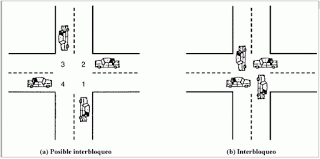
\includegraphics[width=10cm]{figs/01-cruces.png}
  \end{center}

\end{frame}

%---------------------------------------------------------------------
\begin{frame}
  \frametitle{{\em Deadlocks}}

  \ldots u otros nombres menos favorables

  \begin{center}
    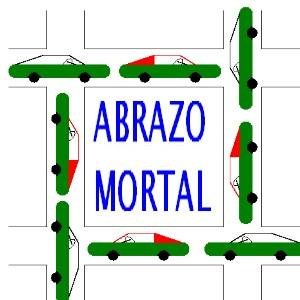
\includegraphics[width=5cm]{figs/01-abrazomortal.jpg}
  \end{center}

  (\#NOT!!)
\end{frame}

%---------------------------------------------------------------------
\begin{frame}
  \frametitle{{\em Deadlocks}}

  Puede verse así:
  
  \begin{center}
    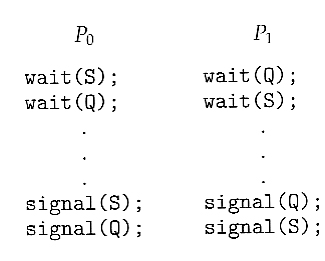
\includegraphics[width=6cm]{figs/01-dealocks-code.jpg}
  \end{center}

\end{frame}

%---------------------------------------------------------------------
\begin{frame}
  \frametitle{{\em Deadlocks}}

  O así:

  \begin{center}
    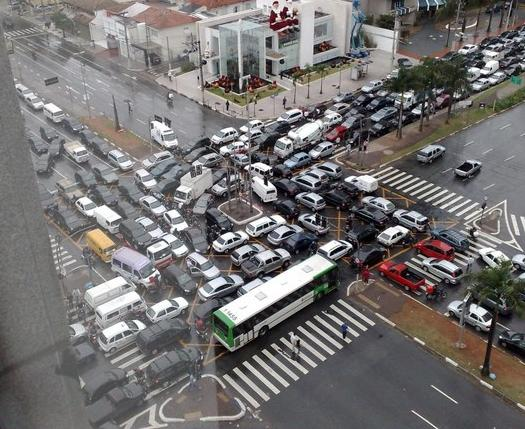
\includegraphics[width=8cm]{figs/01-cruce-gridlock.jpg}
  \end{center}


\end{frame}

%---------------------------------------------------------------------
\begin{frame}
  \frametitle{{\em Deadlocks}}

  ¿Cuándo se producen?
  
  \onslide<2->{Cuando hay {\bf competencia por recursos}}
  
  \onslide<3->{
  Modelo:
  
  \begin{itemize}
    \item Cantidad finita de recursos y de procesos
    \item Distintas clases de recursos (CPU, dispositvo E/S, \ldots)
    \item Cada proceso ejecuta en algún momento estos pasos:
      \begin{itemize}
        \item {\bf Solicitar} recursos ({\em request})
        \item {\bf Utilizar} recurso ({\em use})
        \item {\bf Liberar} recurso ({\em release})
      \end{itemize}
  \end{itemize}
  }

\end{frame}

%---------------------------------------------------------------------
\begin{frame}
  \frametitle{Caracterización de {\em Deadlocks}}

  Condiciones {\em necesarias}
  
  \begin{description}
    \item[{\bf Exclusión mutua}] Existe al menos un recurso {\bf no compartible}
    \item[{\bf Hold and Wait}] Un proceso debe poseer el recurso y esperar otro recurso
    \item[{\bf Ausencia de expropiación}] Los recursos sólo pueden ser liberados voluntariamente
    \item[{\bf Espera circular}] Conjunto $\{P_0, P_1,\ldots,P_n\}$ tal que ``$P_0$ espera a $P_1$'',
                                 ``$P_1$ espera a $P_2$'', \ldots ``$P_n$ espera a $P_0$''
  \end{description}

\end{frame}

%---------------------------------------------------------------------
\begin{frame}
  \frametitle{Grafo de Asignación de Recursos}

  Herramienta para determinar la ocurrencia de {\em deadlocks}
  \begin{block}{Grafo de Asignación de Recursos ({\em Resource-Allocation Graph})}
    Grafo dirigido $G=(V,E)$
    \begin{itemize}
      \item $V = P \cup R$. $P=\{P_1, P_2, \ldots, P_n\}$ son los procesos activos;
                            $R=\{R_1, R_2, \ldots, R_m\}$ son clases de recursos en el sistema
      \item Arista de solicitud. $P_i \to R_j$: $P_i$ está esperando un recurso de clase $R_j$
      \item Arista de asignación. $R_j \to P_i$: Recurso clase $R_j$ ha sido asignado a $P_i$
    \end{itemize}
  \end{block}

\end{frame}

%---------------------------------------------------------------------
\begin{frame}
  \frametitle{Grafo de Asignación de Recursos}

  $P=\{P_1,P_2,P_3\}$
  
  $R=\{R_1,R_2,R_3,R_4\}, |R_1|=1, |R_2|=2, |R_3|=1, |R_4|=3$
  
  $E=\{P_1 \to R_1, P_2 \to R_3, R_1 \to P_2, R_2 \to P_2, R_2 \to P_1, R_3 \to P_3\}$

  \begin{center}
    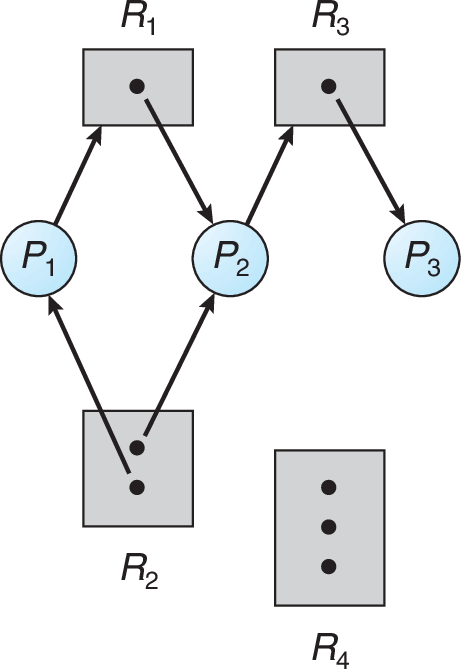
\includegraphics[width=3cm]{figs/01-7_01.pdf}
  \end{center}

  {\em ¿Deadlock?} \ldots \onslide<2->{No (¿por qué?)}

\end{frame}

%---------------------------------------------------------------------
\begin{frame}
  \frametitle{Grafo de Asignación de Recursos}

  \begin{alertblock}{Condición de {\em deadlock}}
    En el grafo de asignación de recursos:
    \begin{itemize}
      \item Si no hay ciclos $\to$ no hay {\em deadlock}
      \item Si hay ciclos $\to$ puede haber {\em deadlock}
    \end{itemize}
  \end{alertblock}
  
  \onslide<2->{
  ¿Y si hay una sola instancia de cada clase de recurso?
  }
  \begin{center}
  \onslide<3->{Ciclo $\Leftrightarrow$ {\em deadlock}}
  \end{center}
    
\end{frame}

%---------------------------------------------------------------------
\begin{frame}
  \frametitle{Grafo de Asignación de Recursos}

  \begin{center}
    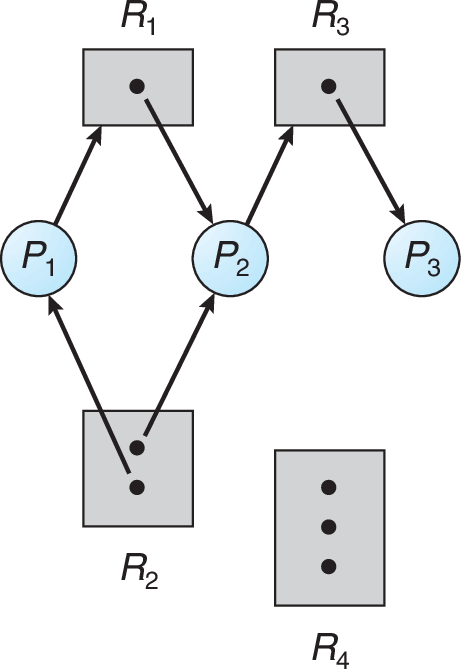
\includegraphics[width=3cm]{figs/01-7_01.pdf}
    $P_3$ solicita $R_2$
    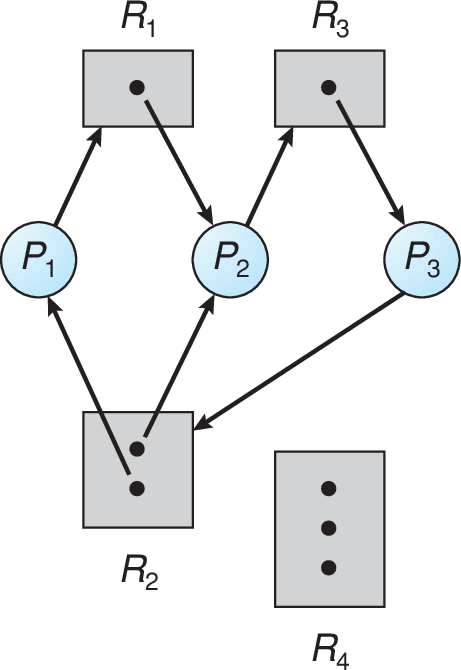
\includegraphics[width=3cm]{figs/01-7_02.pdf}
  \end{center}

  \onslide<2->{¡{\em Deadlock}!}
\end{frame}

%---------------------------------------------------------------------
\begin{frame}
  \frametitle{Grafo de Asignación de Recursos}

  \begin{center}
    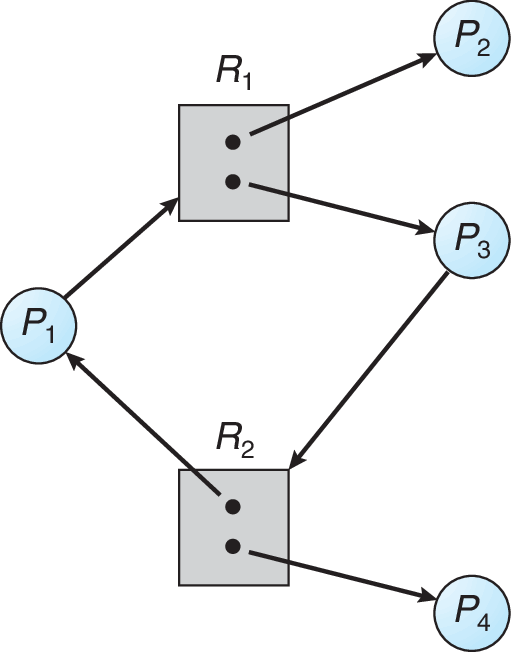
\includegraphics[width=4cm]{figs/01-7_03.pdf}
  \end{center}

  \onslide<2->{¡Ciclo! \ldots}\onslide<3->{ pero sin {\em deadlock}}
\end{frame}

%---------------------------------------------------------------------
\begin{frame}
  \frametitle{¿Como manejar {\em deadlock}s?}

  Tres alternativas:
  \begin{itemize}
    \item Prevenir o evitar llegar a un estado de {\em deadlock}
    \item Permitir el {\em deadlock}, detectarlo, y tomar medidas
    \item Ignorarlo
  \end{itemize}

  \begin{center}
    \includegraphics<2->[width=6cm]{figs/01-avestruces.jpg}
  \end{center}

\end{frame}

%---------------------------------------------------------------------
\begin{frame}
  \frametitle{Prevención de {\em deadlock}s}
  \framesubtitle{Decisión política}

  Asegurar que al menos una de las condiciones {\bf no se cumpla}.
  

  \begin{itemize}
    \item {\bf Impedir ``Exclusión mutua''}. Que todos los recursos sean compartibles.
    \item {\bf Impedir ``Hold-and-wait''}. No ejecutar mientras no se tengan todos los recursos:
          procesos deben solicitar todos los recursos antes de ejecutar ; o bien,
          no permitir solicitudes a procesos que ya tengan recursos asignados
          \begin{itemize}
            \item -Posible subutilización de recursos
            \item -Posible inanición
          \end{itemize}
  \end{itemize}
\end{frame}


%---------------------------------------------------------------------
\begin{frame}
  \frametitle{Prevención de {\em deadlock}s}
  \framesubtitle{Decisión política}

  Asegurar que al menos una de las condiciones {\bf no se cumpla}.
  

  \begin{itemize}
    \item {\bf Impedir ``No expropiación''}. Permitir expropiación.
          Si el proceso tiene recursos, solicita más y no se pueden asignar, entonces
          debe liberar los que ya tiene.
            \begin{itemize}
              \item O bien, quitarle los que otro proceso necesita
              \item Aplicable a recursos cuyo estado se puede recuperar
            \end{itemize}

    \item {\bf Impedir ``Espera circular''}. Que todos los recursos deban ser solicitados en el mismo orden.
          \begin{itemize}
            \item ¿Por qué esto es suficiente?
            \item -La regla debe ser respetada por el programador
            \item FreeBSD incluye objetos {\em witness} que verifican este orden
%Chequear ejemplo Figure 7.5!!
          \end{itemize}
  \end{itemize}
\end{frame}


%---------------------------------------------------------------------
\begin{frame}
  \frametitle{Evitar {\em deadlock}s}
  \framesubtitle{Solución algorítmica}
  
  En lugar de impedir alguna condición ``políticamente'', tomar
  la acción justo antes que ocurra el {\em deadlock}.
  
  \onslide<2->{Require examinar dinámicamente el grafo de asignación de recursos}
  
  \begin{itemize}
    \item<3-> Cada procesos debe especificar la cantidad máxima de recursos que puede pedir
  \end{itemize}
  
  \onslide<4->{
  \begin{exampleblock}{{\bf Estado seguro} ({\em safe state})}
    Un estado es seguro si el sistema puede satisfacer las necesidades de todos los procesos
    en algún orden, y evitar el {\em deadlock}.
    
    Para un conjunto ordenado de procesos $\{P_1, P_2, \ldots, P_n\}$, el estado es seguro
    si cada proceso $P_i$ puede satisfacer su demanda máxima usando los recursos que tiene,
    y los que tienen los procesos $P_j$, $j<i$.
  \end{exampleblock}
  }

\end{frame}

%---------------------------------------------------------------------
\begin{frame}
  \frametitle{Evitar {\em deadlock}s}

  \begin{itemize}
    \item Un estado que no es seguro es \ldots {\bf inseguro}
    \item<2-> Un estado de {\em deadlock} es {\em inseguro}
    \item<3-> No todo estado {\em inseguro} es estado de {\em deadlock}
  \end{itemize}
  
  \begin{center}
    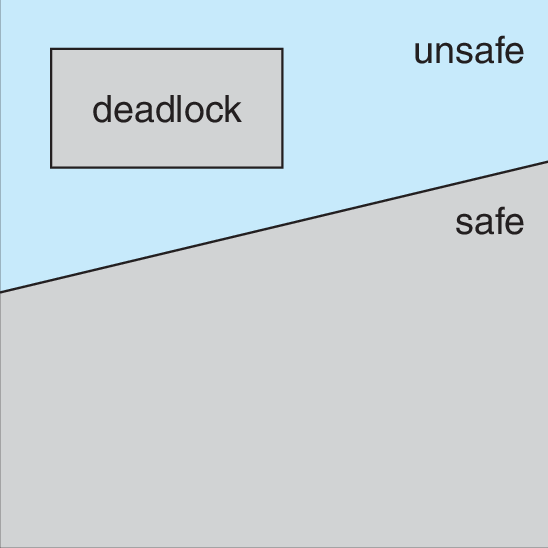
\includegraphics[width=4cm]{figs/01-7_06.pdf}
  \end{center}

  \onslide<4->{
  La política es mantenerse siempre en estados seguros
  }

\end{frame}

%---------------------------------------------------------------------
\begin{frame}
  \frametitle{Evitar {\em deadlock}s}

  Ejemplo: $P=\{P_0,P_1,P_2\}$, $R=\{R_0\}$, $|R_0|=12$
  
  Solicitud máxima: $S_M=\{10,4,9\}$
  
  Solicitud actual: $S_a=\{5,2,2\}$
  
  \begin{center}
    ¿Está el sistema en un estado seguro?
  \end{center}

  \onslide<2->{Sí, ya que existe la secuencia $\langle P_1, P_0, P_2 \rangle$}
  
  \onslide<3->{
  \begin{center}
    ¿Y si a $P_2$ se le asigna un recurso más?
  \end{center}
  }
  
  \onslide<4->{
    {\bf ¡Estado inseguro!} (¿por qué?)
  }  

\end{frame}

%---------------------------------------------------------------------
\begin{frame}
  \frametitle{Evitar {\em deadlock}s}
  \framesubtitle{Volviendo al grafo de asignación de recursos}
  
  Nuevo tipo de arista (existían de solicitud y de asignación):
  
  \onslide<2->{Arista de {\bf demanda}: $P_i\to R_j$ significa que $P_i$ {\em puede} solicitar 
               el recurso $R_j$ en el futuro.}

  \begin{center}
    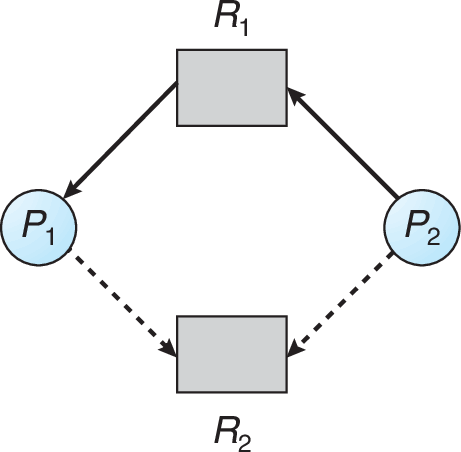
\includegraphics[width=3cm]{figs/01-7_07.pdf}
  \end{center}

  \onslide<3->{Algoritmo: satisfacer solicitud sólo si al satisfacer demanda
               no se obtiene un ciclo}
               
  \onslide<4->{Costo de detectar ciclo con $n$ procesos: }\onslide<5->{$O(n^2)$}
  
\end{frame}

%---------------------------------------------------------------------
\begin{frame}
  \frametitle{Evitar {\em deadlock}s}
  \framesubtitle{Algoritmo del banquero (E.W.Dijkstra, 1977)}

  Analogía: el banquero entrega dinero de manera que pueda satisfacer a todos sus clientes
  
  \begin{itemize}
    \item<2-> Cada proceso debe declarar su máximo de demanda para cada (clase de) recurso,
             que no debe ser mayor que el máximo existente
    \item<3-> El algoritmo sólo asigna recursos si se mantiene dentro de un estado seguro
  \end{itemize}
  
  \onslide<4->{Estructuras: $m$ recursos, $n$ procesos}
  \begin{itemize}
    \item<5-> {\tt Available[m]}, cantidad disponible para cada recurso
    \item<5-> {\tt Max[n][m]}, máxima demanda para cada proceso.
      \begin{itemize}
        \item {\tt Max[i][j]=k}: $P_i$ puede solicitar hasta $k$ instancias de $R_j$
      \end{itemize}
    \item<5-> {\tt Allocation[n][m]}, cantidades asignadas a cada proceso.
      \begin{itemize}
        \item {\tt Allocation[i][j]=k}: $P_i$ tiene $k$ instancias de $R_j$
      \end{itemize}
    \item<5-> {\tt Need[n][m]}, solicitud potencial para cada proceso
      \begin{itemize}
        \item {\tt Need[i][j]=k}: $P_i$ podría pedir hasta $k$ instancias de $R_j$
        \item {\tt Need[i][j] == Max[i][j] - Allocation[i][j]}
      \end{itemize}
  \end{itemize}
  
  
\end{frame}

%---------------------------------------------------------------------
\begin{frame}[fragile]
  \frametitle{Evitar {\em deadlock}s}
  \framesubtitle{Algoritmo del banquero (E.W.Dijkstra, 1977)}

  ¿Cómo saber si estamos en un estado seguro?
  
  \begin{minted}[mathescape,numbersep=5pt,gobble=2,frame=lines,framesep=2mm,fontsize=\scriptsize,linenos=false]{c}
    /** Safety Algorithm **/
    int Work[m] = Available;
    bool Finish[n] = FALSE;
    
    /** encontrar indice $i$ tal que Finish[i]==FALSE y Need[i] $\leq$ Work **/
    while(existe i tal que (!Finish[i] && Need[i] <= Work)) {
      Work = Work + Allocation[i];
      Finish[i] = TRUE;
    }
    for(i=0;i<n;i++) {
      if(Finish[i] == FALSE) {
        return UNSAFE;
      }
    }
    return SAFE;
  \end{minted}
  
  Tiempo de ejecución: \onslide<2->{$O(m \times n^2)$}
  
\end{frame}

%---------------------------------------------------------------------
\begin{frame}[fragile]
  \frametitle{Evitar {\em deadlock}s}
  \framesubtitle{Algoritmo del banquero (E.W.Dijkstra, 1977)}

  ¿Cómo determinar si es posible hacer una asignación de recursos?
  
  Input: {\tt Request[i]}, solicitud de $P_i$
  \begin{minted}[mathescape,numbersep=5pt,gobble=2,frame=lines,framesep=2mm,fontsize=\scriptsize,linenos=false]{c}
    assert(Request[i] <= Need[i]); /** no puede pedir mas de lo que declara **/
    if(Request[i] <= Available) {
      /** Simula una asignacion **/
      Available = Available - Request[i];
      Allocation[i] = Allocation[i] + Request[i];
      Need[i] = Need[i] - Request[i];
      if(safetyAlgorithm() == SAFE) { /** el de la slide anterior **/
        return ALLOCATED;
      }
      else {
        /** deshacer la asignacion **/
        return WAIT;
      }
    }
    else {
      return WAIT;
    }
  \end{minted}
\end{frame}

%---------------------------------------------------------------------
\begin{frame}
  \frametitle{Evitar {\em deadlock}s}
  \framesubtitle{Algoritmo del banquero (E.W.Dijkstra, 1977)}

  Ejemplo: $P=\{P_0,P_1,P_2,P_3,P_4\}, R=\{R_A,R_B,R_C\}$
  
  $|R_A|=10, |R_B|=5, |R_C|=7$
  
  Estado actual:
  \[
  \begin{array}{c|c|c|c|}
   \textbf{Alloc} & A & B & C \\ \hline
   P_0 & 0 & 1 & 0 \\ \hline
   P_1 & 2 & 0 & 0 \\ \hline
   P_2 & 3 & 0 & 2 \\ \hline
   P_3 & 2 & 1 & 1 \\ \hline
   P_4 & 0 & 0 & 2 \\ \hline
  \end{array}
  \qquad 
  \begin{array}{c|c|c|c|}
   \textbf{Max} & A & B & C \\ \hline
   P_0 & 7 & 5 & 3 \\ \hline
   P_1 & 3 & 2 & 2 \\ \hline
   P_2 & 9 & 0 & 2 \\ \hline
   P_3 & 2 & 2 & 2 \\ \hline
   P_4 & 4 & 3 & 3 \\ \hline
  \end{array}
  \qquad
   \begin{array}{c|c|c|c|}
   \textbf{Need} & A & B & C \\ \hline
   P_0 & 7 & 4 & 3 \\ \hline
   P_1 & 1 & 2 & 2 \\ \hline
   P_2 & 6 & 0 & 0 \\ \hline
   P_3 & 0 & 1 & 1 \\ \hline
   P_4 & 4 & 3 & 1 \\ \hline
  \end{array}
  \]
  $\textbf{Available}=\{3,3,2\}$
  
  El estado actual es {\bf safe}, ¿por qué? \onslide<2->{({$\langle P_1,P_3,P_4,P_2,P_0 \rangle$})}
  
  \begin{itemize}
    \item<3-> Ejecutar {\em request} de $P_1$: {\tt Request[1]=\{1,0,2\}}
    \item<3-> Ejecutar {\em request} de $P_4$: {\tt Request[4]=\{3,3,0\}}
    \item<3-> Ejecutar {\em request} de $P_0$: {\tt Request[0]=\{0,2,0\}}
  \end{itemize}
\end{frame}


%---------------------------------------------------------------------
\begin{frame}
  \frametitle{Detectar {\em deadlock}s}

  Si no se toma ninguna acción previa, pueden ocurrir {\em deadlocks}
  
  \onslide<2->{Se necesita:}
  
  \begin{itemize}
    \item<3->{Algoritmo para detectar {\em deadlocks}}
    \item<3->{Algoritmo para resolver {\em deadlocks}}
  \end{itemize}
  
  Costo de detectar ciclos en grafo de asignación de $n$ procesos: $O(n^2)$

  \begin{center}
    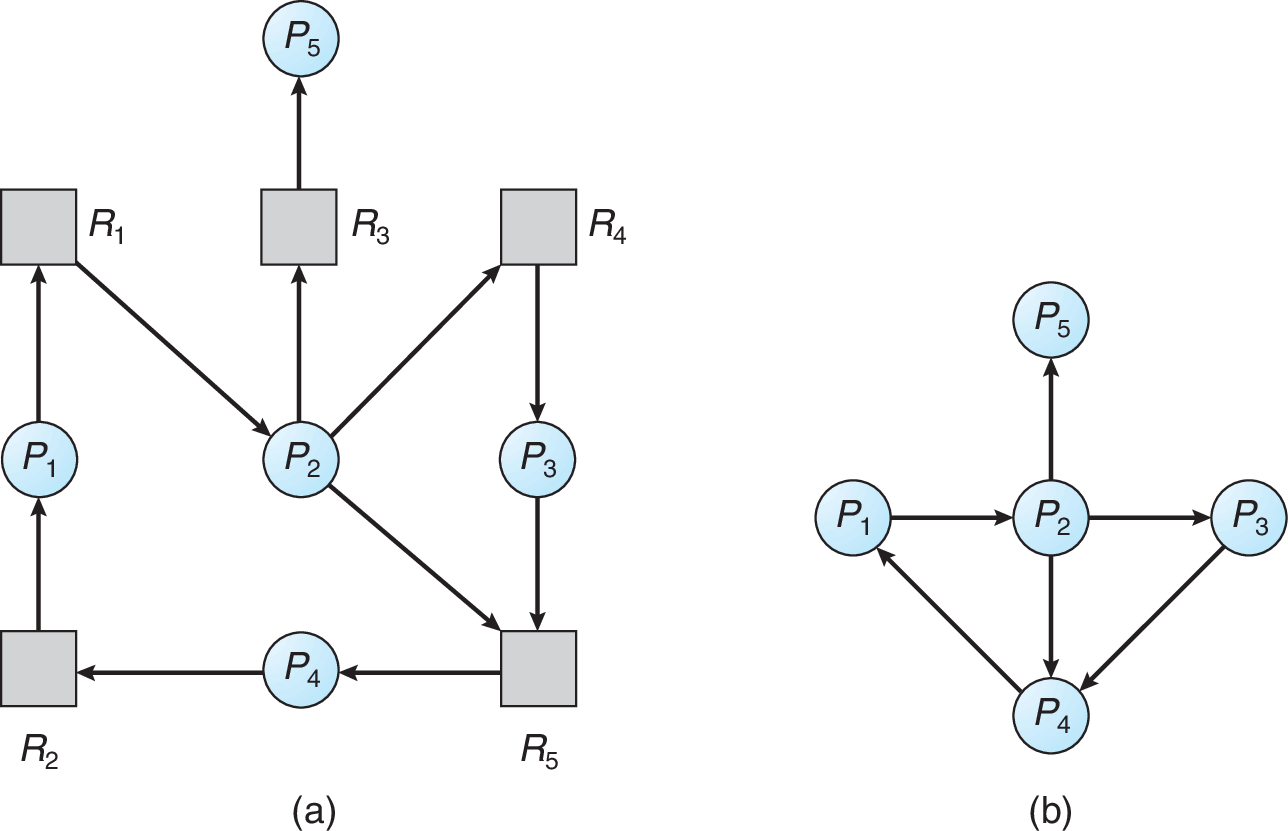
\includegraphics[width=6cm]{figs/01-7_09.pdf}
  \end{center}

\end{frame}


%---------------------------------------------------------------------
\begin{frame}
  \frametitle{Detectar {\em deadlock}s}
  \framesubtitle{Pero con múltiples instancias por recurso}
  
  Algoritmo de detección de {\em deadlock} basado en el banquero
  
  \onslide<2->{Estructuras: $m$ recursos, $n$ procesos}
  \begin{itemize}
    \item<2-> {\tt Available[m]}, cantidad disponible para cada recurso
    \item<2-> {\tt Allocation[n][m]}, cantidades asignadas a cada proceso.
      \begin{itemize}
        \item {\tt Allocation[i][j]=k}: $P_i$ tiene $k$ instancias de $R_j$
      \end{itemize}
    \item<2-> {\tt Request[n][m]}, solicitud actual para cada proceso
      \begin{itemize}
        \item {\tt Request[i][j]=k}: $P_i$ solicita $k$ instancias de $R_j$
      \end{itemize}
  \end{itemize}
\end{frame}

%---------------------------------------------------------------------
\begin{frame}[fragile]
  \frametitle{Detectar {\em deadlock}s}
  \framesubtitle{Pero con múltiples instancias por recurso}
 
  Detección de {\em deadlock}
  
  \begin{minted}[mathescape,numbersep=5pt,gobble=2,frame=lines,framesep=2mm,fontsize=\scriptsize,linenos=false]{c}
    /** Deadlock detection algorithm **/
    int Work[m] = Available; bool Finish[n];
    for(i=0;i<n;i++)
      if(Allocation[i] != 0) Finish[i] = FALSE;
      else                   Finish[i] = TRUE;
    /** encontrar indice $i$ tal que Finish[i]==FALSE y Request[i] $\leq$ Work **/
    while(existe i tal que (!Finish[i] && Request[i] <= Work)) {
      Work = Work + Allocation[i];
      Finish[i] = TRUE;
    }
    /** todos pueden terminar? **/
    for(i=0;i<n;i++)
      if(Finish[i] == FALSE) return DEADLOCKED;
    return NOT_DEADLOCKED;
  \end{minted}
  Todos los procesos para los cuales {\tt Finish[i]==FALSE} están en {\em deadlock}
  
  Tiempo de ejecución: \onslide<2->{$O(m \times n^2)$}

\end{frame}

%---------------------------------------------------------------------
\begin{frame}
  \frametitle{Detectar {\em deadlock}s}

  Ejemplo: $P=\{P_0,P_1,P_2,P_3,P_4\}, R=\{R_A,R_B,R_C\}$
  
  $|R_A|=10, |R_B|=5, |R_C|=7$
  
  Estado actual:
  \[
  \begin{array}{c|c|c|c|}
   \textbf{Alloc} & A & B & C \\ \hline
   P_0 & 0 & 1 & 0 \\ \hline
   P_1 & 2 & 0 & 0 \\ \hline
   P_2 & 3 & 0 & 3 \\ \hline
   P_3 & 2 & 1 & 1 \\ \hline
   P_4 & 0 & 0 & 2 \\ \hline
  \end{array}
  \qquad 
  \begin{array}{c|c|c|c|}
   \textbf{Req} & A & B & C \\ \hline
   P_0 & 0 & 0 & 0 \\ \hline
   P_1 & 2 & 0 & 2 \\ \hline
   P_2 & 0 & 0 & 0 \\ \hline
   P_3 & 1 & 0 & 0 \\ \hline
   P_4 & 0 & 0 & 2 \\ \hline
  \end{array}
  \]
  $\textbf{Available}=\{0,0,0\}$
  
  El estado actual es {\bf NOT DEADLOCKED}, ¿por qué? \onslide<2->{({$\langle P_0,P_2,P_3,P_1,P_4 \rangle$})}
  
  \begin{itemize}
    \item<3-> Ejecutar {\em request} de $P_2$: {\tt Request[2]=\{0,0,1\}}
  \end{itemize}
\end{frame}

%---------------------------------------------------------------------
\begin{frame}
  \frametitle{Recuperación ante {\em deadlock}s}

  OK, hemos detectado el {\em deadlock} (so what?)
  
  \onslide<2->{Dos caminos\ldots}
  \begin{itemize}
    \item<3-> {\bf Matar un proceso} ¿Cuál?
      \begin{itemize}
        \item<4-> Todos (solución drástica)
        \item<5-> Uno a la vez hasta resolver el {\em deadlock}
          \begin{itemize}
            \item Criterio 1: La cantidad mínima
            \item Criterio 2: El de menor ``costo''
          \end{itemize}
      \end{itemize}
    \item<6-> {\bf Expropiar recursos}
      \begin{itemize}
        \item ¿A quién?
        \item {\bf Rollback}
      \end{itemize}
  \end{itemize}

\end{frame}

%---------------------------------------------------------------------
\begin{frame}
  \frametitle{Recuperación ante {\em deadlock}s}
  \framesubtitle{Algunos puntos importantes}

  \begin{itemize}
    \item {\em Deadlock}: dos o más procesos esperando indefinidamente por un evento
          que sólo puede ser producido por uno de ellos mismos.
          \begin{itemize}
            \item Requieren: recursos no compartibles, no expropiables, ``retención-y-espera'',
                  y espera circular.
            \item Si se impide una de estas condiciones, no se puede producir {\em deadlock}
          \end{itemize}
    \item Tres alternativas de manejo:
      \begin{itemize}
        \item Prevenir (que nunca pueda ocurrir), o evitar (esquivarlo antes que pase)
        \item Permitirlo y recuperarse. Desafío: resolver con el menor ``daño'' posible
        \item Ignorarlo
      \end{itemize}
    \item Algoritmo del banquero (Dijkstra, 1977), evita que el proceso llegue a un {\em estado inseguro}
    \item Sistema en {\em estado seguro} no puede estar en {\em deadlock}
  \end{itemize}

\end{frame}

%---------------------------------------------------------------------
\begin{frame}
  \frametitle{Administración de Procesos}
  \framesubtitle{¿Qué debemos recordar?}
 
  \begin{itemize}
    \item Procesos: programa+recursos, administrados por el S.O. mediante {\em syscall}s
    \item {\em Threads}: unidad básica de ejecución visible al programador o al S.O.
    \item Sincronización de {\em threads} permite que puedan ejecutar eficientemente, sin bloquearse,
          y sin provocar inconsistencias en los datos compartidos
    \item Algoritmos de {\em scheduling} permiten seleccionar eficientemente el próximo proceso/{\em thread} a ejecutar
    \item Se debe evitar caer en situación de {\em bloqueo mutuo}
  \end{itemize}


\end{frame}

\end{document}